\documentclass{article}

\usepackage[preprint]{neurips_2025}

\usepackage[utf8]{inputenc}
\usepackage[T1]{fontenc}
\usepackage{hyperref}
\usepackage{url}
\usepackage{booktabs}
\usepackage{amsfonts}
\usepackage{amsmath}
\usepackage{nicefrac}
\usepackage{microtype}
\usepackage{graphicx}
\usepackage{subcaption}
\usepackage{multirow}
\usepackage{xcolor}
\usepackage{enumitem}

\title{Reading and Writing an Agent's Belief About Its Own Next Action}

\author{%
  Anonymous Author(s) \\
  Affiliation \\
  \texttt{email} \\
}

\newcommand{\qvec}{q}
\newcommand{\kent}{\kappa^{\mathrm{ent}}}
\newcommand{\kfin}{\kappa^{\mathrm{fin}}}
\newcommand{\kmar}{\kappa^{\mathrm{mar}}}
\newcommand{\Tstab}{T^{\mathrm{stab}}}
\newcommand{\Tverb}{T^{\mathrm{verb}}}
\newcommand{\Tperm}{T^{\mathrm{perm}}}

\begin{document}

\maketitle

\begin{abstract}
When a language-model agent reasons before acting, at what point does it actually decide,
what is that decision made of, and can it be changed? We measure a
\emph{forced-answer belief} --- the distribution the model would emit over its four
available actions if forced to answer now --- at every one of $98{,}310$ prefixes of the
chains of thought that \texttt{gpt-oss-20b} produces while solving key--door gridworlds.
Three findings follow. First, the agent typically \emph{names an action before it decides
on one}: the median first action mention arrives at $25\%$ of the way through the chain,
the answer stops changing at $49\%$, and a median $51\%$ of the chain (524 tokens) is
generated after the answer has permanently settled; only $36\%$ of decisions stabilise
before their first verbalisation. Second, the belief is highly legible from the residual
stream --- held-out Spearman $0.771 \pm 0.009$ across five trajectory-grouped folds,
against $0.371$ for a positional baseline restricted to information the probe's inputs
could contain --- and it decomposes into two nearly orthogonal channels, \emph{strength}
and \emph{content}, which we separate in four independent ways. Third, and in sharp
contrast, the belief is remarkably hard to \emph{direct}: rank-1 activation steering flips answers at perturbations
comparable to the state itself, but no more often than a norm-matched random direction
($0.135$ vs $0.130$), deleting an
entire attention or MLP sub-block perturbs the answer without aiming it, transplanting a whole
$12{\times}2880$ activation window --- one of the $24$ layers the probe reads --- redirects
only $20.8\%$ of cases, and an
explicit instruction to disregard the reasoning recovers $0.14\%$ of the belief mass it
was asked to restore. We argue this read/write asymmetry is the central object: the belief
is redundantly encoded and continuously reconstructed from context rather than stored at a
site. Along the way we report a data-integrity failure --- a key--value-cache-reusing
scorer produced labels that disagree with a cache-free re-extraction on $93.5\%$ of rows,
and with an independent API scorer on $29.8\%$ of top actions --- whose diagnosis we
recommend as routine practice for forced-answer measurements.
\end{abstract}

\section{Introduction}

A language-model agent that reasons before acting produces a long chain of thought and
then a single action. The chain is often treated as an explanation of the action, but the
relationship between the two is exactly what is in question: the reasoning may construct
the decision, report a decision already made, or run alongside it \citep{turpin2023,
lanham2023}. Answering this requires a measurement of what the model would do at
intermediate points, not just at the end.

We adopt a simple such measurement, extending the ``early answering'' protocol of
\citet{lanham2023}: at any cut $t$ of a chain of thought, append a fixed suffix that forces
the model into its answer format, and read the distribution over the four action tokens.
Where early answering records the agreement rate of a truncated answer, we keep the full
four-way distribution at every prefix, which is what makes strength and content separable
and gives the clocks below their resolution. This \emph{forced-answer belief} $\qvec_s(t) \in \Delta^3$ is a
functional of the model at that cut, requires no probe, and --- because the four actions
are single tokens --- is exactly normalisable. Sweeping $t$ gives a belief trajectory per
decision, and sweeping decisions gives a corpus: $98{,}310$ prefixes over $1{,}276$
decisions in $95$ trajectories of \texttt{gpt-oss-20b} in key--door gridworlds.

Prior work has measured when models commit to answers, but almost entirely in
\emph{question answering with binary or few-option answers}, using either behavioural
log-odds \citep{commit2026} or probes trained to predict eventual correctness
\citep{temporal2025}. We work in an \emph{agentic} setting with a full four-way belief
simplex, a spatial task whose evidence accumulates gradually, and --- crucially --- with
both the behavioural and the representational sides measured on the same objects, so that
we can ask not only \emph{when} the belief settles but \emph{what it is made of} and
\emph{whether it can be moved}.

\paragraph{Contributions.}
\begin{enumerate}[leftmargin=1.4em,itemsep=1pt,topsep=2pt]
\item \textbf{Agentic commitment dynamics} (\S\ref{sec:when}). Three per-decision clocks
--- verbalisation, argmax stabilisation, permanent high commitment --- in that median
order ($0.25 < 0.49 < 0.65$). The model usually names an action before it settles on one,
and half the chain is post-decision. The switch hazard declines smoothly with no sharp
boundary, and commitment is imperfectly absorbing: at commitment $0.95$, $8.9\%$ of states
still switch later.

\item \textbf{A legible two-channel code} (\S\ref{sec:what}). Commitment is decodable at
$0.771 \pm 0.009$ Spearman from activations alone, far above a positional bar we argue is
the correct one ($0.371$) and above an oracle baseline that is given information no causal
state can contain ($0.644$). Belief \emph{strength} and belief \emph{content} occupy
nearly orthogonal linear directions of the same layers, established four independent ways.

\item \textbf{A read/write asymmetry} (\S\ref{sec:move}). Four intervention families ---
rank-1 steering, sub-block deletion, full-window transplantation, and natural-language
instruction --- can damage the belief but cannot direct it. We argue this is evidence
about the encoding, not about our interventions.

\item \textbf{Methodology} (\S\ref{sec:setup}, \S\ref{sec:pitfalls}). A fair-versus-oracle
positional-control framework; a demonstration that probe-occlusion importance and
model-ablation importance disagree and must not be conflated; and a label-integrity
failure with a cheap triangulation test that catches it.
\end{enumerate}

\section{Setup}
\label{sec:setup}

\paragraph{Agent, task, corpus.} \texttt{gpt-oss-20b} (24 blocks, residual width 2880)
navigates 2-D key--door gridworlds; the action set is
$\mathcal{A}=\{\textsc{up},\textsc{down},\textsc{left},\textsc{right}\}$. A \emph{decision
step} $s$ comprises a prompt $x_s$ (serialised world state), a chain of thought $c_s$ of
$N_s$ tokens, and the action $a_s$ taken. The corpus has $95$ trajectories, $1{,}276$
decisions, $98{,}310$ prefixes; median $N_s \approx 1{,}500$. Cuts are thinned to at most $80$ per decision, so the gap
between consecutive cuts has median $20$ tokens but ranges from $1$ to $150$ and is coarser
in longer chains. Because $\Tstab$ is verified only at sampled cuts, it is a \emph{lower}
bound and the post-decision tail is correspondingly an \emph{upper} bound; this bias runs
against the reported length effect, which is therefore conservative.

\paragraph{Forced-answer belief.} With $\sigma$ the fixed 12-token suffix that opens the
answer JSON (validated token-exactly at load),
\begin{equation}
\qvec_s(t) \;=\; \mathrm{softmax}\!\left(\mathrm{logits}_M\!\left(x_s \,\|\, c_s[1{:}t] \,\|\, \sigma\right)\big|_{\mathcal{A}}\right) \in \Delta^3 .
\end{equation}
We use normalised-entropy commitment $\kent(q) = 1 - H(q)/\log 4$, commitment to the
eventual action $\kfin_s(t) = \qvec_s(t)(a_s)$, and margin $\kmar = q_{(1)}-q_{(2)}$.
\emph{Progress} is $\tau = t/N_s$. The suffix is used only to define this functional; it is
never an input to any probe. A prefix is \emph{pre-verbal} if its cut precedes the first
action word in the chain ($31{,}723$ prefixes, $32.3\%$); all pre-verbal claims use this
subset.

\paragraph{Activations and probe contract.} We store residual states at all 24 block
outputs for the last $W{=}12$ genuine chain-of-thought tokens, projected $2880\to512$ by a
fixed seeded scaled-orthogonal matrix (hash-pinned). Probes obey a strict contract: frozen
backbone; activation-only inputs; $<\!10^6$ readout parameters; five trajectory-grouped
outer folds with zero trajectory overlap, verified at load; no task features, no future
tokens, no forced-suffix states.

\paragraph{A model-selection artifact we disclose.} Probe selection optimises validation
commitment Spearman only, so folds 2 and 3 selected an auxiliary action-loss weight of zero
and shipped untrained action heads (held-out top-action accuracy $0.34$/$0.24$ versus
${\approx}0.50$ elsewhere). Commitment results are unaffected; every action-head quantity we
report uses folds 0, 1 and 4 only.

\paragraph{Fair versus oracle positional baselines.} Commitment rises with position, so a
probe could score well by decoding position alone. We distinguish two baselines. The
\textbf{fair bar} may use only the prefix token index $t$ --- the only positional quantity
the probe's inputs could encode. \textbf{Oracle bars} may additionally use $N_s$ or
$\tau$, which \emph{no causal state at cut $t$ can contain}, because the remaining tokens
do not yet exist. Papers that control for ``progress'' are typically using an oracle; we
report both and treat only the fair bar as a threshold.

\paragraph{Label integrity.}
\label{sec:labels}
Our first scorer reused a key--value cache across prefixes. Its labels disagree with
re-extracted labels on $93.5\%$ of rows (mean row-wise $\max_a|\Delta q_a| = 0.235$;
top-action agreement $0.719$). Three independent paths adjudicate: against an independent
API scorer the re-extracted labels agree at $0.971$ (mean $\max|\Delta q| = 0.026$) versus
$0.702$ for the cached ones; against fully cache-free forward passes, $0.982$; and in the
terminal region ($\tau > 0.9$) the re-extracted top action equals the action actually taken
in $97.9\%$ of prefixes versus $91.5\%$ for the cached ones. We stress that the
\emph{final} prefix does not discriminate --- both regimes score $1.000$ there, because the
corruption vanishes as the chain ends --- which is precisely why the failure survived
casual inspection. All results below use the adjudicated labels.
Because the corruption is invisible without a second scoring path --- it produces
plausible, smoothly varying, wrong numbers --- we recommend this triangulation as routine
for any forced-answer measurement. Quantitatively, the corrupted labels \emph{delayed}
apparent commitment (median lock-in $0.288 \to 0.190$) and \emph{inflated} apparent
switching ($8.40 \to 6.04$ switches per decision).

\section{When does the agent commit?}
\label{sec:when}

\paragraph{Three clocks.} For each decision we define $\Tverb$, the progress of the first
action word in the text; $\Tstab$, the first cut after which $\arg\max \qvec_s$ never
changes again; and $\Tperm(c)$, the first cut after which $\kfin_s \ge c$ always holds.
Their medians are ordered
\begin{equation}
\Tverb = 0.253 \;<\; \Tstab = 0.494 \;<\; \Tperm(0.8) = 0.648 ,
\end{equation}
and only $35.6\%$ of decisions satisfy $\Tstab < \Tverb$ (Figure~\ref{fig:clocks}, left).
The agent typically \emph{names} an action before it \emph{settles} on one; early mentions
are candidates under deliberation, not announcements.

\paragraph{Half the chain is post-decision.} The post-commitment tail $1-\Tstab$ has median
$0.506$ (524 tokens; mean 887). Short chains have the largest relative tails (shortest
quartile median stabilisation $0.316$ versus $0.596$ for the longest): when the answer is
easy, most of the chain follows the decision. This is the agentic analogue of the
``epiphenomenal'' tail reported for question answering \citep{boundary2026}, obtained with
a belief functional rather than early-exit accuracy.

\paragraph{At the decision, the chain stops parsing and starts re-deriving.} We
characterise the post-$\Tstab$ text three ways; all ratios are per-decision means with
trajectory-clustered bootstrap CIs, and every keyword class passed an author-labelled
precision check (protocol, weighting conventions, and robustness table in
Appendix~\ref{app:lexicon}). \emph{Discovered vocabulary:} a fully data-driven contrast
(log-odds with informative Dirichlet prior; \citealp{monroe2008}) shows the terms rising
most after stabilisation are path enumeration (``steps'', coordinate pairs, ``then'',
bare direction words), answer machinery (``action'', ``output''), optimality talk
(``shorter'', ``minimal''), and the conclusion marker ``thus''; the terms falling most
are map-parsing vocabulary (``row'', ``col'', raw numerals, the grid symbols,
``walls'', ``indices'', ``map''). \emph{Keyword classes:} checking vocabulary rises
$3.73\times$ $[3.37, 4.15]$, conclusion markers $10.9\times$, sequencing $2.60\times$,
and coordinate pairs $1.41\times$, while grid nouns fall to $0.37\times$ and
self-correction markers to $0.86\times$ $[0.79, 0.94]$; answer-naming uses of direction
words are essentially tail-exclusive ($29$ versus $1751$ hits). \emph{Event alignment:}
comparing each class's local density jump at $\Tstab$ against a placebo that redraws the
stabilisation point from other chains of similar length, checking spikes \emph{at} the
decision ($+0.43$/1k versus placebo $[+0.17, +0.35]$, $p = 0.01$), grid nouns collapse
there ($-1.61$ versus $[-0.97, -0.38]$), and coordinates jump ($+5.6$ versus
$[+1.2, +3.6]$), whereas conclusion markers show no excess at $\Tstab$ ($+0.03$ versus
$[+0.14, +0.29]$): they are anchored to the end of the chain, not to the decision.
Before the decision the model parses the world; at the decision it stops parsing and
re-walks the solution in concrete coordinates with explicit checking; only at the end
does it name the answer (Figure~\ref{fig:tail}, right). The tail is re-derivation and
checking, not continued deliberation --- and not mere restatement either.

\paragraph{But the tail is not cheaply cuttable.} We swept 63 genuinely prospective
early-exit rules --- margin threshold $c$, persistence $k$ consecutive prefixes above $c$,
and a minimum-token floor, none using the unknowable $N_s$ --- and took the Pareto
frontier. The best rule reaches $93.3\%$ agreement with the full-chain action at $28.3\%$
mean token savings; only 2 of 63 rules exceed $90\%$ and \emph{none} reaches $95\%$
(Figure~\ref{fig:tail}, left). Debouncing is essential: exiting at the first threshold
crossing scores $42.2\%$, because the belief makes confident transient excursions to the
wrong action. Compared with the ${\sim}55\%$ reported cuttable for question answering
\citep{boundary2026}, the agentic setting is markedly less compressible at comparable
fidelity.

\paragraph{Dynamics: position is a credibility amplifier.} The per-cut switch hazard
declines monotonically with progress ($0.133 \to 0.019$ across deciles) with no sharp
boundary, and commitment is imperfectly absorbing: conditional on current commitment, the
probability of a later switch falls from ${\approx}1$ below $0.35$ to $0.089$ in the top
decile (Figure~\ref{fig:hazard}). We asked whether the belief \emph{screens off} position.
In an additive model it appears to: adding progress to margin changes held-out AUC from
$0.8474$ to $0.8452$. That conclusion would be wrong. An interaction-capable model does
gain ($0.8471 \to 0.8520$), because the position effect \emph{reverses sign} across belief
levels --- in the lowest margin quintile the hazard \emph{rises} with progress
($0.242 \to 0.370$), in the highest it falls roughly tenfold ($0.0156 \to 0.0016$) --- and
the two cancel additively (Figure~\ref{fig:hazint}). Position is therefore not redundant
given the belief; it multiplies the belief's credibility. A decision still unsettled deep
into its chain is in a genuinely unstable regime.

\paragraph{Belief change is anchored.} Following the sentence-level counterfactual analysis
of \citet{anchors2025}, consecutive prefixes differ by one generation chunk,
so per-transition total variation attributes belief change to spans of text. Change is concentrated, with an exponential tail: the top $5\%$ of transitions carry $37.0\%$ of all belief movement, and the
median decision concentrates $28.0\%$ of its movement in its top three transitions
(Figure~\ref{fig:clocks}, right). These anchors are switch events ($75.0\%$ coincide with an
argmax change versus a $7.9\%$ base rate) and $40.8\%$ of them \emph{reduce} commitment.
Concentration predicts early settling: Spearman(top-3 share, $\Tstab$) $=-0.510$.
Chunks containing no action, spatial, plan, or correction vocabulary are $4.2\times$
depleted among anchors. A resampling test of whether anchors are causal forks was
inconclusive at our sample size (dispersion ratio $1.26$, $p=0.32$, $n=20$ per arm); we
report it as underpowered rather than negative.

\begin{figure}[t]
  \centering
  \begin{subfigure}[b]{0.40\textwidth}
    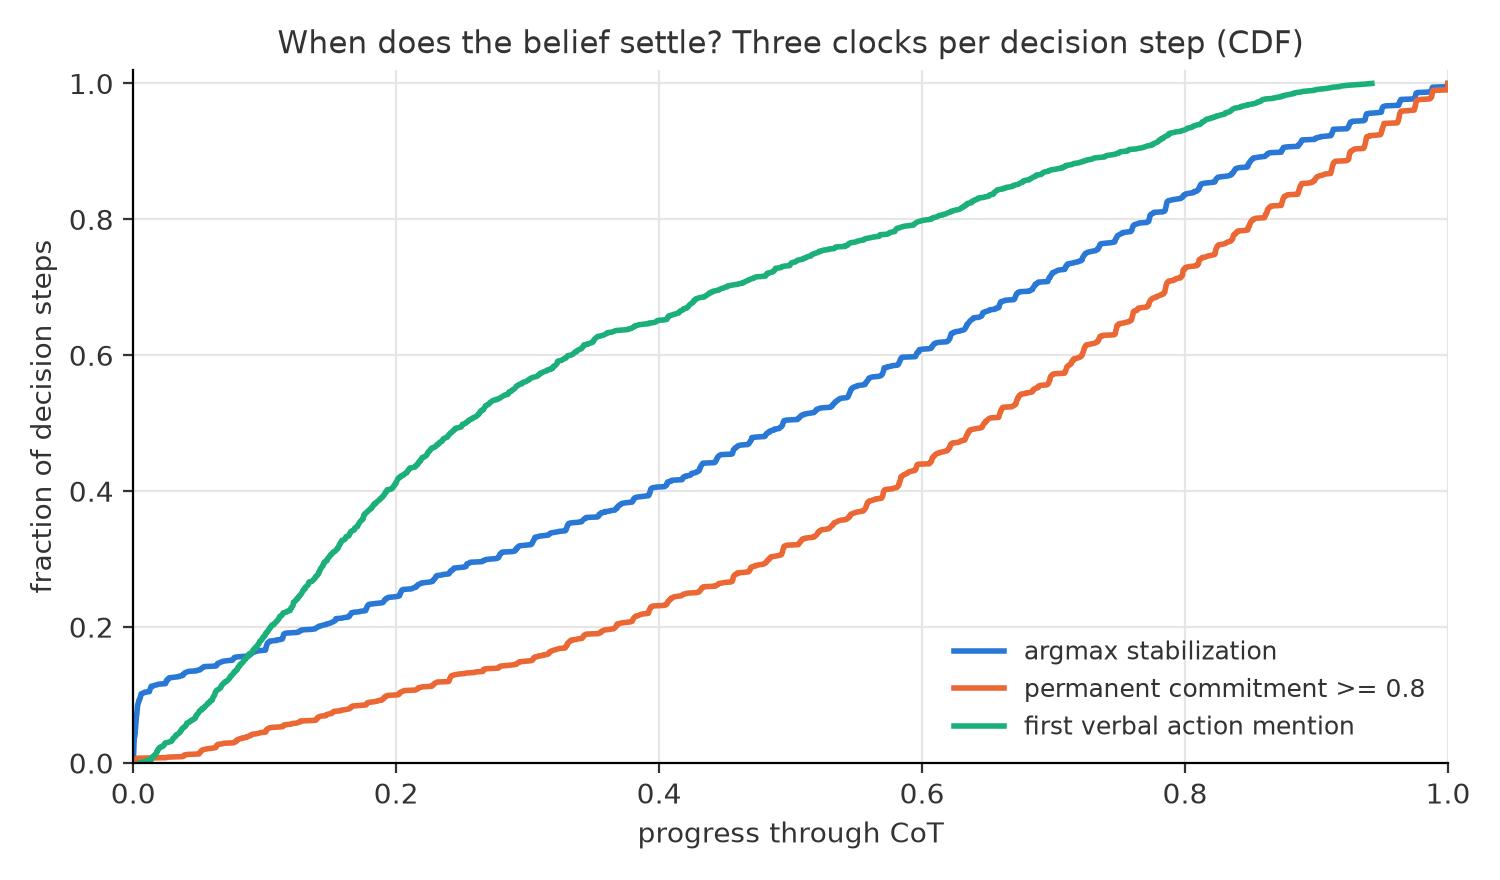
\includegraphics[width=\textwidth]{figures/clocks.png}
  \end{subfigure}
  \hfill
  \begin{subfigure}[b]{0.40\textwidth}
    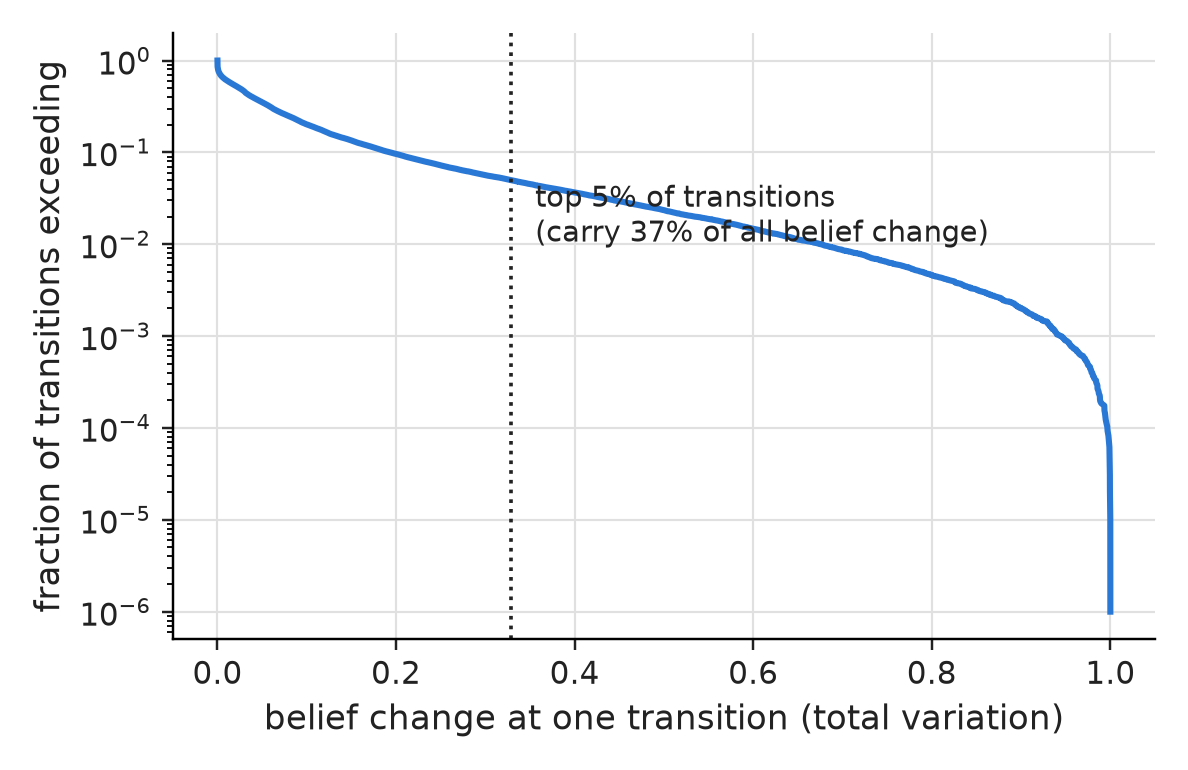
\includegraphics[width=\textwidth]{figures/anchors.png}
  \end{subfigure}
  \caption{\textbf{Left:} cumulative distributions of the three per-decision clocks.
  Verbalisation precedes stabilisation, which precedes permanent high commitment.
  \textbf{Right:} belief change per transition is highly concentrated --- the survival
  function is shown on a log scale, and the top $5\%$ of transitions carry $37\%$ of all movement.}
  \label{fig:clocks}
\end{figure}

\begin{figure}[t]
  \centering
  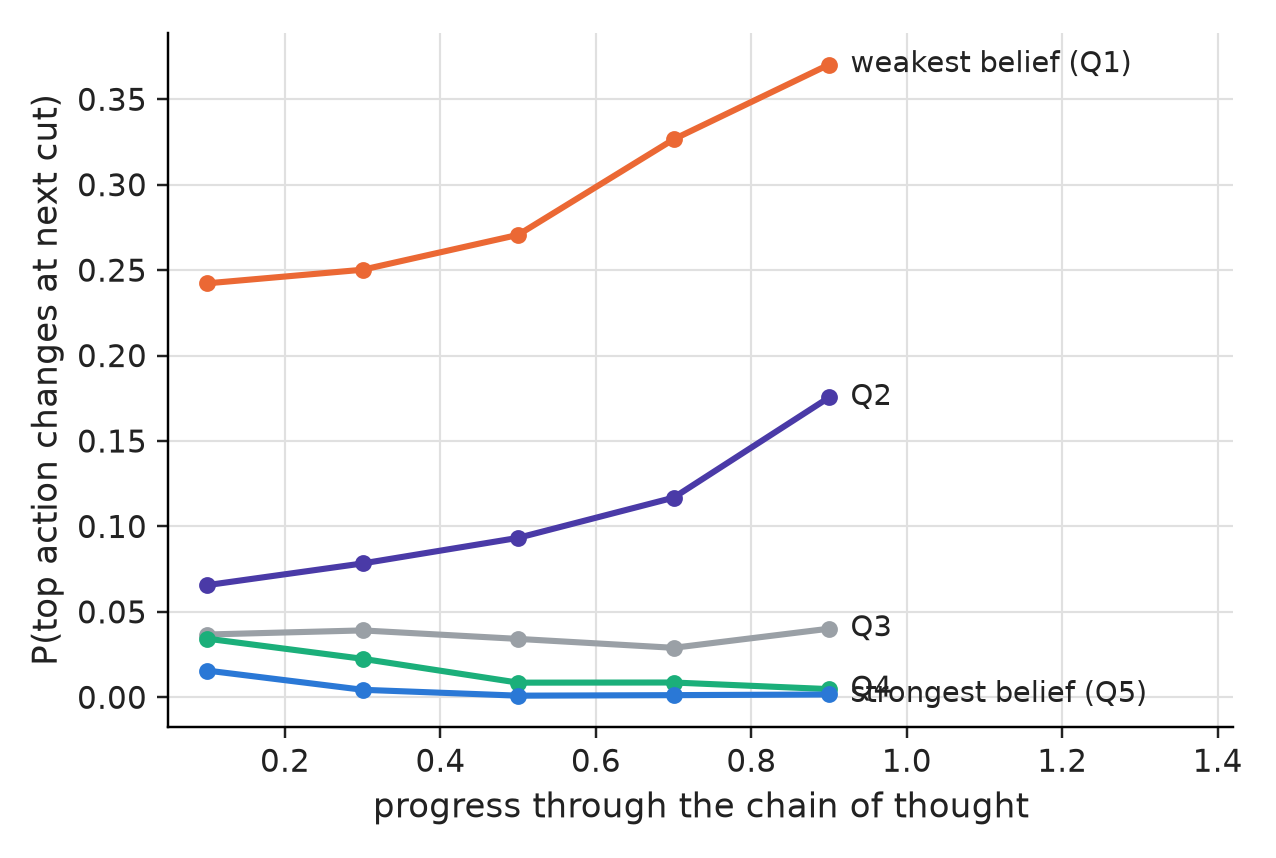
\includegraphics[width=0.76\textwidth]{figures/hazard_interaction.png}
  \caption{Switch hazard against progress \emph{within margin quintiles}. The curves fan in
  \emph{opposite} directions: weakly held beliefs become more volatile as the chain
  proceeds, strongly held ones become more final. An additive model sees these cancel and
  wrongly concludes that position is redundant given the belief. The marginal hazard,
  which declines monotonically, is in Figure~\ref{fig:hazard}.}
  \label{fig:hazint}
\end{figure}

\begin{figure}[t]
  \centering
  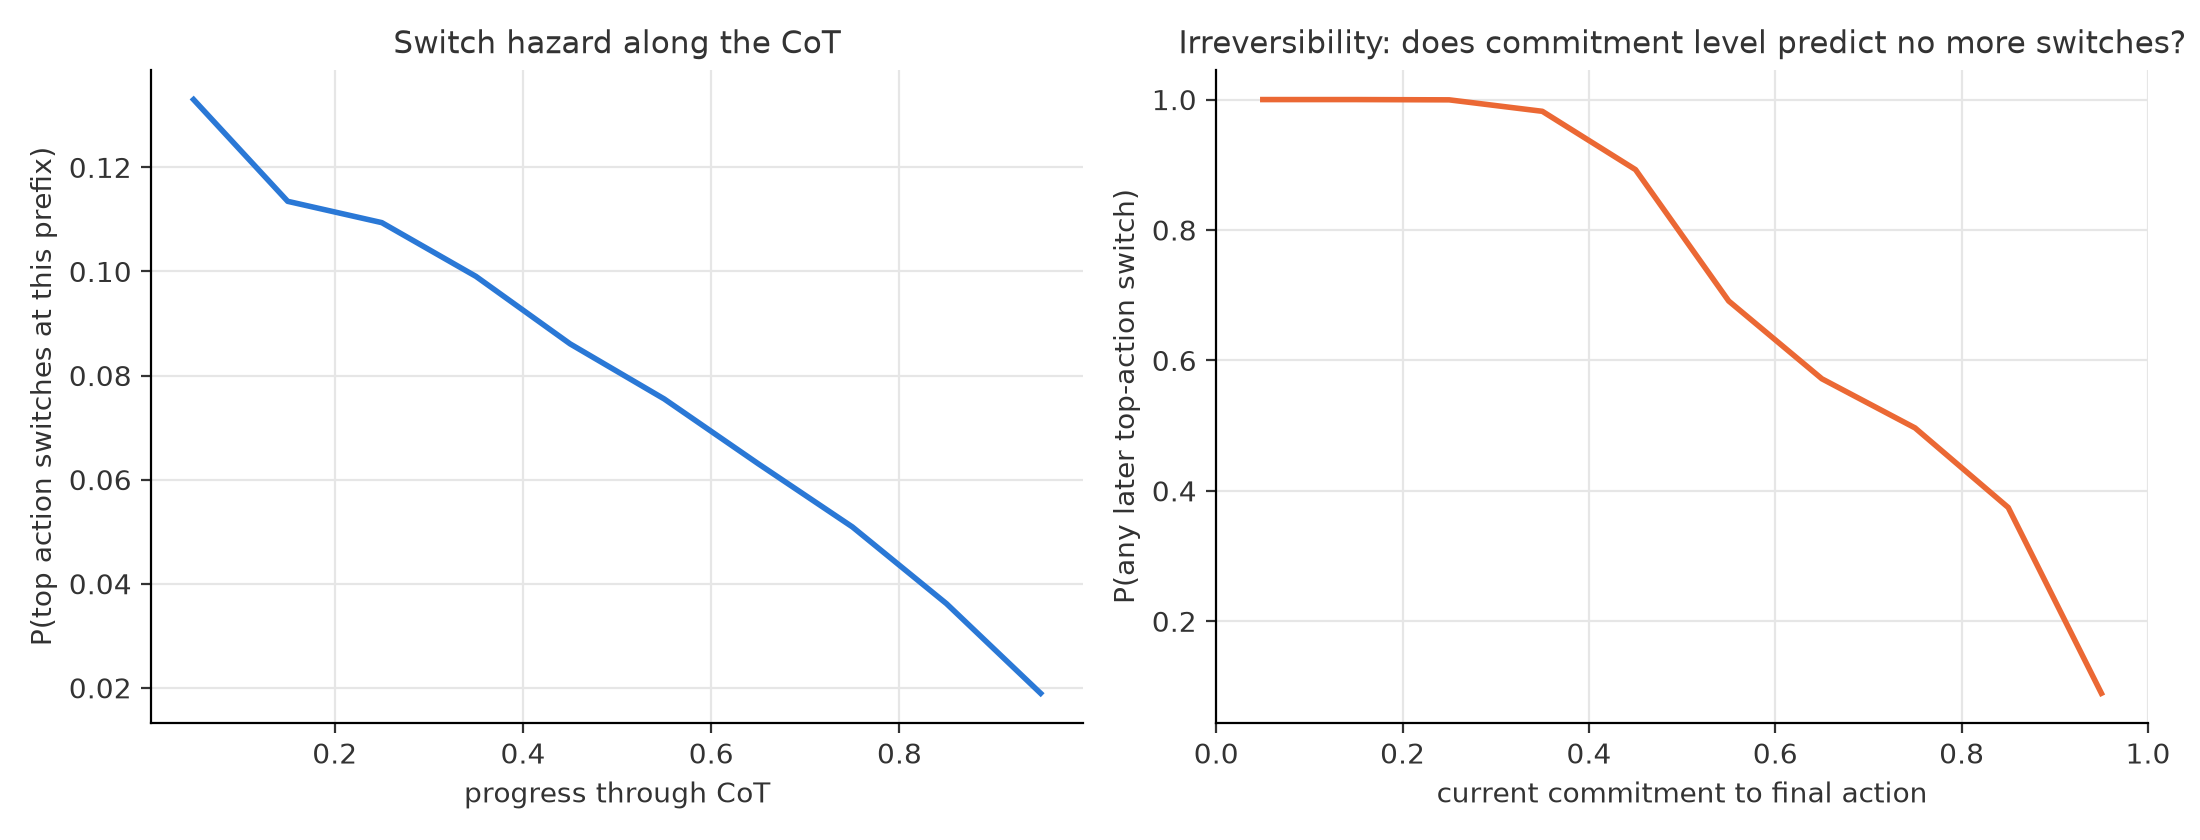
\includegraphics[width=0.58\textwidth]{figures/hazard.png}
  \caption{\textbf{Left:} the probability that the top action changes at the next cut falls
  smoothly with progress; there is no sharp boundary in aggregate. \textbf{Right:}
  conditional on current commitment, the probability of any later switch --- high
  commitment strongly predicts, but does not guarantee, finality.}
  \label{fig:hazard}
\end{figure}

\section{What is the belief made of?}
\label{sec:what}

\paragraph{Commitment is legible and is not position.} A probe reading mask-pooled
chain-of-thought window activations predicts held-out $\kent$ at Spearman
$\mathbf{0.771 \pm 0.009}$ over five trajectory-grouped folds ($R^2 = 0.509$; high/low AUC
$0.957$), against $0.371 \pm 0.015$ for the fair positional bar, $0.644$ for a progress oracle and $0.660$
for a progress-plus-length oracle (Table~\ref{tab:probes}). The signal survives inside fixed progress
bins ($0.52$--$0.71$) where the positional baseline collapses and turns negative
($0.334 \to -0.319$), so it is not position in disguise.

\paragraph{No layer-transition code.} We tested the hypothesis that commitment lives in
layer-to-layer \emph{transitions} by giving a transformer the depth axis as a sequence. It
never beats simple mean-pooling over layers in any fold ($\Delta$ Spearman $-0.016$,
bootstrap CI $[-0.021,-0.011]$), and adjacent-layer difference features add nothing. The
information is in the layers, not in their transitions.

\begin{table}[t]
  \centering
  \small
  \caption{Held-out prediction of normalised-entropy commitment, five trajectory-grouped
  outer folds. Oracle baselines receive the chain's total length, which no causal state at
  cut $t$ can contain; only the fair bar is a legitimate threshold.}
  \label{tab:probes}
  \begin{tabular}{lccc}
    \toprule
    Method & Spearman & SD & $R^2$ \\
    \midrule
    Mean-over-layers readout (best)      & \textbf{0.7715} & 0.0094 & 0.509 \\
    Concatenated-layers readout          & 0.7675 & 0.0091 & 0.506 \\
    Depth-sequence transformer           & 0.7576 & 0.0097 & 0.496 \\
    Best single layer                    & 0.7474 & 0.0437 & 0.463 \\
    Final layer only                     & 0.7045 & 0.0103 & 0.405 \\
    \midrule
    \textit{Oracle:} progress + length spline & 0.6600 & 0.0131 & 0.393 \\
    \textit{Oracle:} progress                 & 0.6435 & 0.0105 & 0.370 \\
    \textit{Fair bar:} token index            & 0.3710 & 0.0154 & 0.201 \\
    \bottomrule
  \end{tabular}
\end{table}

\paragraph{Strength and content are separable channels.} Measuring both targets with the
\emph{same} instrument at every layer (ridge for commitment, balanced logistic for the top
action, on identical pooled features), both are decodable everywhere and peak in the same
mid-to-late band --- action at layers 13--18 (balanced accuracy $0.521$ at L17 versus a
$0.331$ bar), commitment at 13--15 (Spearman $0.669$ at L15 versus $0.343$) --- with a
small but 5-of-5-fold consistent interaction favouring depth for content ($+0.046$;
Figure~\ref{fig:layerwise}). The two are not separated by \emph{depth}. They are separated
\emph{within} layers, though we state the geometry carefully: the commitment direction
places on average $3.2\%$ of its squared norm inside the 3-d action subspace, which is
largely disjoint but is still $5.4\times$ an isotropic chance level of $3/512 = 0.6\%$ (at L10 it is $1.0\%$, near chance).
Overlap is lower through the mid-to-late band than in early layers, but the minima (L10,
L16) are not precisely the decoding peaks (L15, L17), so we claim the band-level trend
only. The functional test is the stronger evidence: Projecting out the action subspace
changes commitment decoding by $<0.004$ Spearman, and removing the commitment direction
changes action decoding by $<0.005$ balanced accuracy, in every fold
(Figure~\ref{fig:geometry}).

Three further measurements, sharing no methodology with the above, find the same split
(Figure~\ref{fig:strengthcontent}):
\begin{enumerate}[leftmargin=1.4em,itemsep=1pt,topsep=2pt]
\item A decoder trained to recover \emph{which} action is favoured is nearly uninformative
about \emph{how strongly}: its implied confidence correlates with true commitment at
$\rho \in [-0.125, +0.043]$ across representations. Giving it a learned multiplicative gain
--- which does improve the fit, and does so only when the gain direction is learned rather
than random --- lifts this only to $+0.12$ to $+0.18$, against $0.771$ for a probe trained
on commitment directly.
\item Before a single reasoning token exists, the prompt-final state already determines the
belief ($R^2 = 0.673$ at L18; balanced accuracy $0.508$ versus $0.25$ chance; the prior is
stark, with \textsc{right} favoured in $79.5\%$ of decisions). Measured consistently on the true
labels, its \emph{strength} predicts when the decision will settle ($\rho = -0.341$) while
\emph{which} action it favours does not ($\rho = -0.039$). We flag that the dissociation
does not appear decoder-side: predicted strength and predicted content perform alike
($-0.044$ vs $-0.054$), which bounds how much of this is representational rather than
behavioural.
\item The commitment direction transfers to a different task. Holding the answer interface
fixed but replacing gridworlds with arithmetic and logic questions --- four options
labelled with the same four tokens, stated to be arbitrary names --- a commitment direction
frozen from gridworld training reaches Spearman $0.515$ with the new task's commitment at
layer 13, against a $0.384$ positional bar and a $0.612$ ceiling from refitting on the new
task: $84\%$ of the ceiling with no new fitting (Figure~\ref{fig:counterfactual}, right). At layer 3 the
transfer is large but sign-inverted ($-0.514$), so the early-layer axis is not the same
quantity.
\end{enumerate}
Commitment therefore behaves like a general confidence code that is largely independent of
what the confidence is about.

\begin{figure}[t]
  \centering
  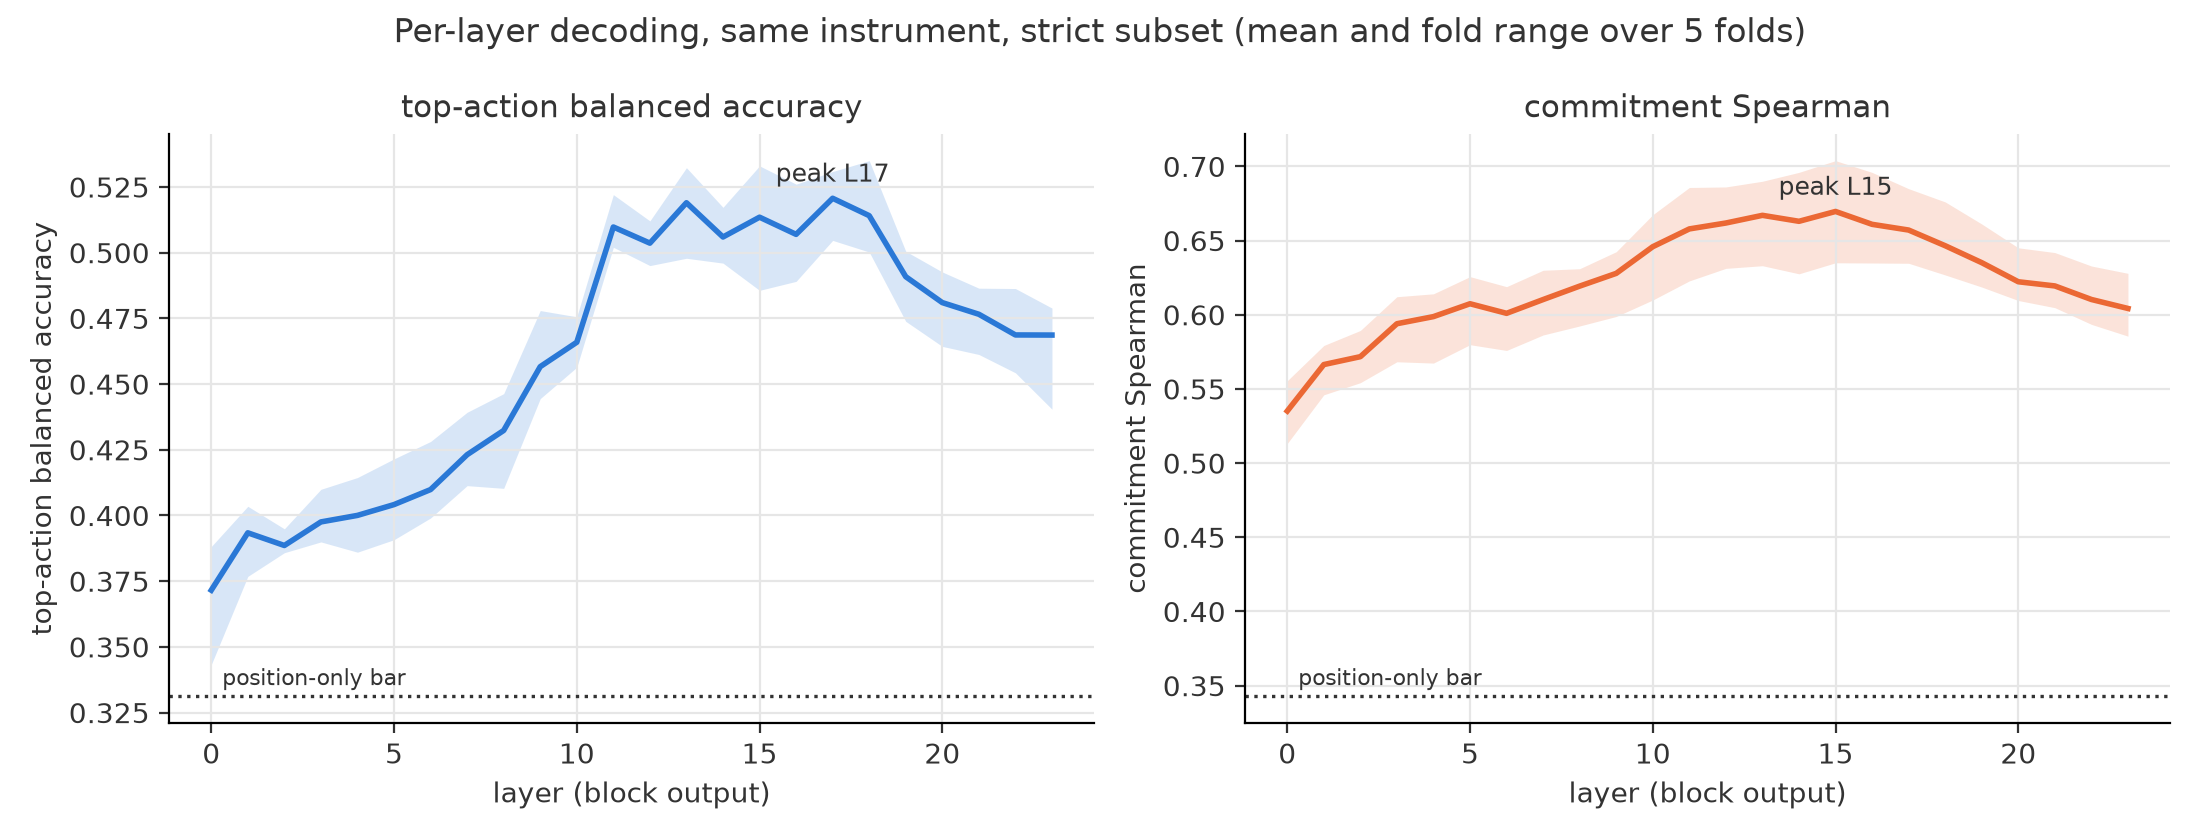
\includegraphics[width=0.76\textwidth]{figures/layerwise.png}
  \caption{Per-layer decoding of the top action and of commitment, measured with the same
  instrument on the same pooled activations, pre-verbal prefixes. Band is the range over
  five folds; dotted line is the fair positional bar. Both quantities peak in the same
  mid-to-late band; they are not separated by depth.}
  \label{fig:layerwise}
\end{figure}

\begin{figure}[t]
  \centering
  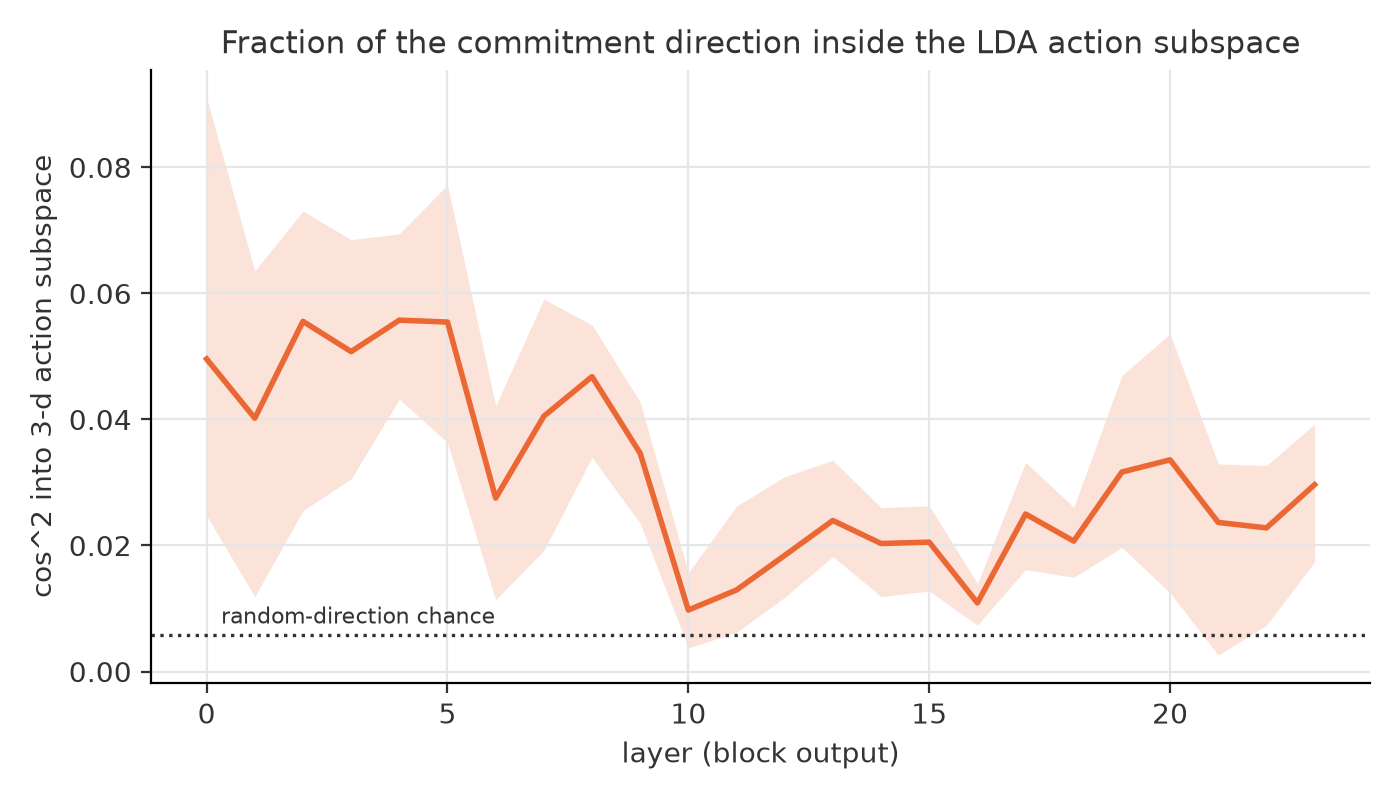
\includegraphics[width=0.44\textwidth]{figures/geometry.png}
  \caption{The fraction of the commitment direction lying inside the action subspace, by
  layer, against an isotropic chance level. Overlap is lower through the mid-to-late band
  than in early layers, though the minima do not coincide precisely with the decoding peaks.}
  \label{fig:geometry}
\end{figure}

\begin{figure}[t]
  \centering
  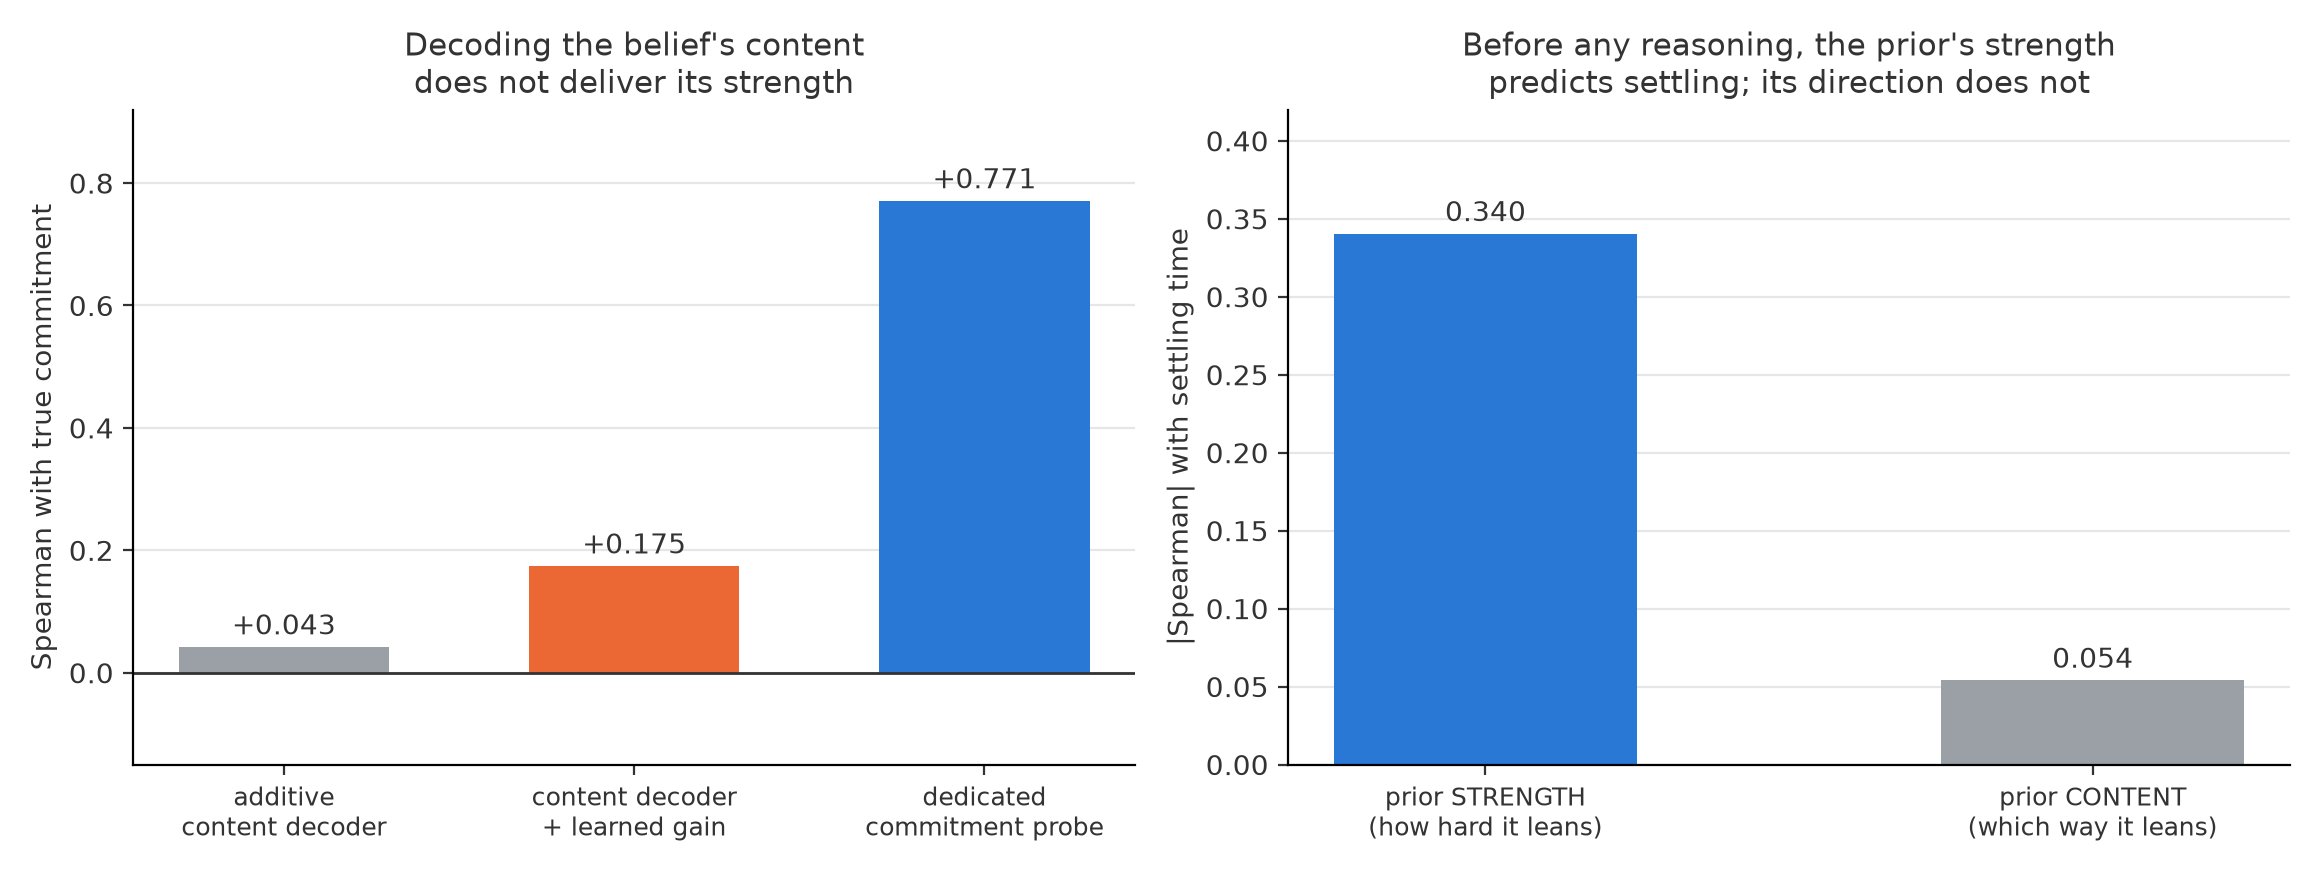
\includegraphics[width=0.70\textwidth]{figures/synthesis_strength_vs_content.png}
  \caption{Two further measurements of the strength/content dissociation, neither relying
  on layer geometry. \textbf{Left:} a decoder trained to recover \emph{which} action is
  favoured knows almost nothing about \emph{how strongly} it is favoured, with or without a
  learned multiplicative gain, against a probe trained on commitment directly.
  \textbf{Right:} before any reasoning exists, how strongly the prompt-final state already
  leans predicts when the answer will settle, while which way it leans does not.}
  \label{fig:strengthcontent}
\end{figure}

\section{Can the belief be moved?}
\label{sec:move}

\paragraph{The belief tracks the reasoning text, not the world state.} We paired the prompt
of decision $A$ with a chain-of-thought prefix from a decision $B$ whose agent took a
different action, cutting at ${\sim}10/50/90\%$ of $B$'s chain, and scored 396 such pairs
plus 396 congruent controls with fully independent forward passes. The belief follows the
foreign reasoning: $\qvec(a_B) \in [0.598, 0.673]$ against $\qvec(a_A) \in [0.129, 0.165]$,
already at the earliest cut (Figure~\ref{fig:counterfactual}). The prompt is not inert ---
with congruent context the model follows the chain's conclusion at $0.985$ late in the
chain versus $0.689$ under conflict --- but the missing mass disperses rather than
returning to $a_A$.

\paragraph{Four ways to try to move it, all largely unsuccessful.}
Table~\ref{tab:interventions} reports each intervention family at its single most effective
setting, split into whether it changed the answer \emph{at all} and whether it changed the
answer to the \emph{intended} one.

\begin{table}[t]
  \centering
  \small
  \caption{Interventions on the belief, each at its best condition (a maximum over
  $4$--$28$ cells, which biases the ``changed answer'' column upward). Wilson $95\%$
  intervals in brackets. The finding is the \emph{level}, not the gap: no intervention
  redirects the answer in more than a fifth of cases. Note that when full-window
  transplantation does work it aims well ($0.208$ of $0.250$), so ``damage without aim'' is
  not the right summary of that row.}
  \label{tab:interventions}
  \begin{tabular}{llccc}
    \toprule
    Intervention & Scope & $n$ & Changed answer & Changed to target \\
    \midrule
    Rank-1 steering ($\|\Delta\|{=}\|h\|$) & 1 of 2880 dims, 12 tok, 1 layer & 96 & 0.146 [0.09,0.23] & 0.135 [0.08,0.22]\rlap{$^\dagger$} \\
    Delete attention or MLP block   & whole sub-block, 1 layer & 24 & 0.292 [0.15,0.49] & n/a\rlap{$^\ddagger$} \\
    Transplant window state         & $12\times2880$ dims, 1 of 24 layers & 24 & 0.250 [0.12,0.45] & 0.208 [0.09,0.41] \\
    Instruct model to ignore chain  & natural language & 396 & 0.058 [0.04,0.09] & 0.010 (net $-0.005$) \\
    \bottomrule
    \multicolumn{5}{l}{\footnotesize $^\dagger$ norm-matched random control reaches 0.130 [0.09,0.19]; Fisher $p=1.00$. $^\ddagger$ no target is defined for a deletion.}
  \end{tabular}
\end{table}

\emph{Steering.} Injecting the decoder-defined commitment or action directions (lifted to
the residual stream through the stored projection) into the probe's own 12-token window
produces no effect distinguishable from a norm-matched random direction. We scale the
injection relative to the token state, $\|\Delta\| = \alpha\|h\|$, and sweep
$\alpha \in \{0.1, 0.25, 0.5, 1\}$ over layers $10/15/18$ ($32$ prefixes; $96$ trials per
cell for the decoder directions, $192$ for the control). Perturbations of this size
\emph{do} change the answer, and increasingly so with $\alpha$ --- but the random direction
changes it just as often:

rate of arriving at the \emph{intended} action, action direction versus norm-matched
random control (Wilson $95\%$): $\alpha=0.25$, $0.052$ [0.02,0.12] vs $0.036$ [0.02,0.07]
($p=0.54$); $\alpha=0.5$, $0.104$ [0.06,0.18] vs $0.052$ [0.03,0.09] ($p=0.14$);
$\alpha=1$, $0.135$ [0.08,0.22] vs $0.130$ [0.09,0.19] ($p=1.00$, Fisher).

At $\alpha = 1$ the perturbation is as large as the state it edits and flips $13.5\%$ of
answers --- statistically indistinguishable from the $13.0\%$ produced by a random vector of
the same norm. This is the cleanest form of the paper's claim: at magnitudes where the
intervention demonstrably \emph{does} something, the decoder direction is no better at
choosing \emph{what} it does than noise. We note two remaining limits: the directions lie in
the fixed random $512$-of-$2880$ subspace the probe reads, and we ran no positive-control
direction known to steer this model.

\emph{Sub-block deletion.} Skipping an entire attention or MLP sub-block at one layer --- a
strict upper bound on head-level ablation --- costs at most $0.097$ nats of KL over 28
conditions. This intervention \emph{does} flip answers ($29\%$ at its worst site), but it
has no target; it is damage, not control.

\emph{Transplantation.} We built a nested ladder in which a donor prefix with a different
answer supplies replacement content, and only the number of transplanted dimensions varies:
rank-1 along the commitment axis, rank-1 along the donor's action direction, rank-3 along
the action subspace, and the full $12\times2880$ window. Rank-1 and rank-3 are exactly
inert (flip rate $0.000$ everywhere). Full-window replacement --- overwriting every number
the probe reads --- redirects only $20.8\%$ of pairs at its best layer.

\emph{Instruction.} Appending an explicit disavowal (``the reasoning above was copied from
a different maze $\ldots$ decide using only the map'') to the mismatched pairs recovers
$0.14\%$ of the belief mass the mismatch costs; $4/396$ rows gain the prompt's action as
argmax while $6/396$ lose it, a net $-0.005$. The effect is statistically reliable but
numerically trivial ($72.2\%$ of rows move in the predicted direction, Wilcoxon
$p = 1.3{\times}10^{-8}$), and congruent controls move a comparable amount in the harmful
direction --- a small generic loss of confidence, not a reattribution.

\paragraph{Interpretation.} One caveat on the comparison: $0.771$ is a \emph{strength}
readout, whereas the intervention rates concern \emph{action identity}, whose matched
read-side number is the more modest $0.521$ balanced accuracy against a $0.331$ bar
(\S\ref{sec:what}). The asymmetry holds within the strength channel too --- steering moves
$\kent$ by at most $0.006$ in any cell. With that said: no intervention we applied can point
the belief at a chosen action more than a fifth of the time, and the only
one that does anything overwrites the probe's entire input. The natural reading is that the
belief is \emph{redundantly encoded and continuously reconstructed from context} --- the
prompt and the earlier chain --- rather than stored in the window where it is most legible.
This is the belief-valued analogue of the self-repair and Hydra effects documented for
component ablation \citep{mcgrath2023, wang2023ioi}: what we add is that it holds for a
graded, decodable quantity under targeted rather than merely destructive edits. It should be
read as such an instance, not as a new phenomenon.
The window the probe reads is where the belief is \emph{visible}, not where it \emph{lives}
(Figure~\ref{fig:readwrite}).

\begin{figure}[t]
  \centering
  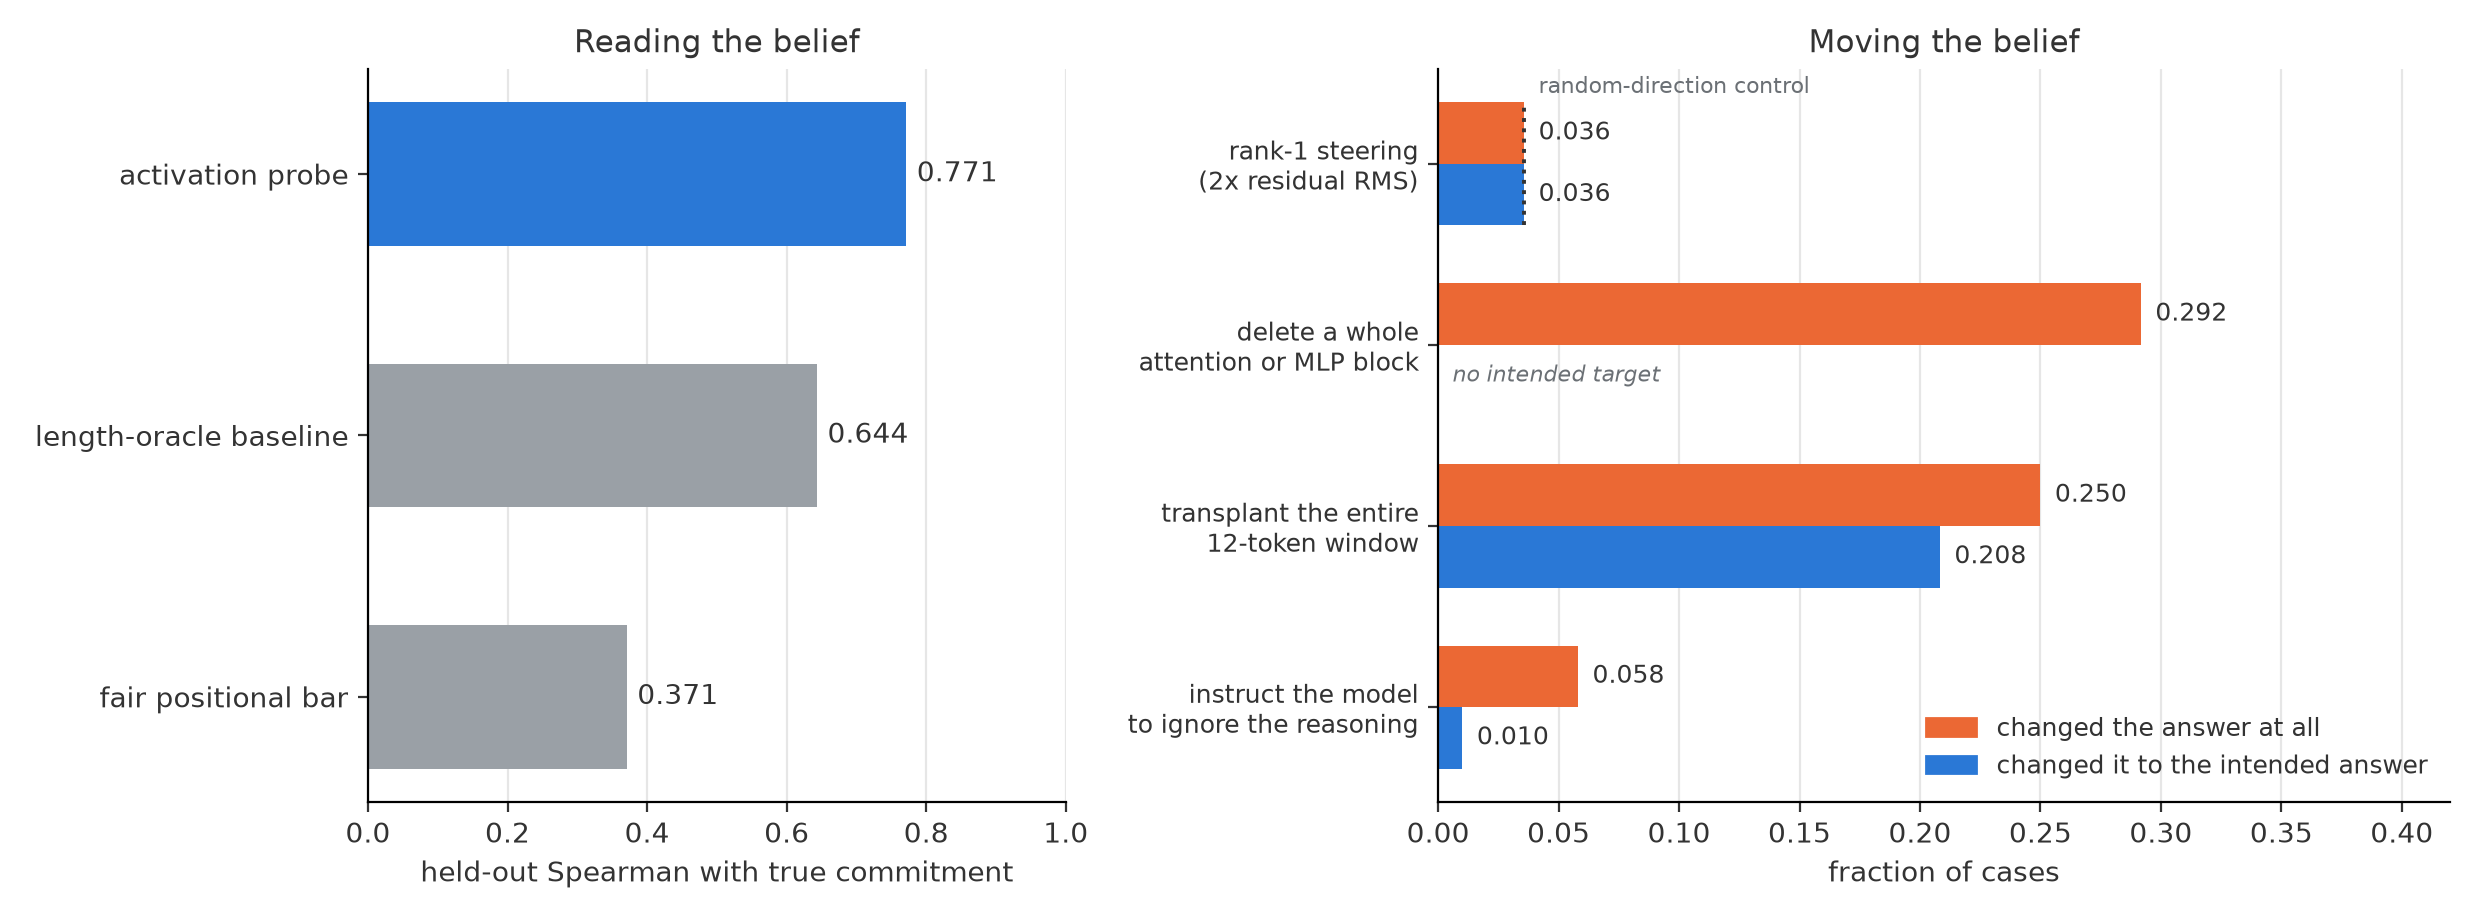
\includegraphics[width=0.76\textwidth]{figures/synthesis_read_write_asymmetry.png}
  \caption{The read/write asymmetry. Left: decodability of commitment against the fair
  positional bar and an oracle baseline. Right: four intervention families, each at its
  best setting, separated into changing the answer at all versus changing it to the
  intended answer.}
  \label{fig:readwrite}
\end{figure}

\section{Two methodological pitfalls}
\label{sec:pitfalls}

\paragraph{Probe-occlusion importance is not causal importance.} Occluding layers of a
trained probe identifies layer 10 as uniquely load-bearing in four of five folds (mean
Spearman drop $0.093$; other salient layers are fold-specific). It is tempting to read this
as a claim about the model. It is not: ablating layer 10's \emph{attention in the model}
damages the belief \emph{less} ($0.049$ nats) than ablating layer 0's ($0.086$), and no
sub-block anywhere exceeds $0.097$. Layer 10 is where the belief becomes linearly
\emph{readable} --- it coincides with a sharp jump in decodability from L10 to L11 --- not
where it is computed. The two importance measures answer different questions and here they
disagree.

\paragraph{An additive control can confirm a false hypothesis.} As shown in
\S\ref{sec:when}, testing whether the belief screens off position with an additive model
returns the ``expected'' null, while the true structure is an interaction with opposite
signs in different regimes. Screening-off claims should be tested with models that can
represent interactions.

\section{Related work}

\paragraph{When models commit.} \citet{commit2026} track finite-answer log-odds in
delayed-verdict binary tasks and find preference stabilisation $17$--$31$ tokens before the
answer is parseable; \citet{boundary2026} identify a commitment boundary after which
reasoning is largely epiphenomenal, cutting up to ${\sim}55\%$ of the trace;
\citet{temporal2025} predict eventual correctness from early hidden states. All are
question-answering settings with behavioural or correctness targets. We contribute the
agentic, four-way, full-distribution version, and find both a familiar phenomenon (a large
post-decision tail) and an unfamiliar one (that tail is not cheaply cuttable, because early
confidence is frequently misplaced).

\paragraph{Beliefs in the residual stream.} \citet{shai2024} show that transformers
linearly embed the belief-state geometry of their data-generating process. Our supervised
projections recover the action signal that unsupervised methods miss --- in our data the
leading principal components track token position ($|r|$ up to $0.57$), not action --- but
the behavioural simplex geometry does not transfer to activation space, which we report as
an informative negative for naive geometric transfer.

\paragraph{Belief--action gaps.} \citet{broken2026} show in strategic games that beliefs
are decodable yet weakly drive actions. Our gap is complementary and temporal: the belief
that generates the action is itself driven by the reasoning text rather than the world
state, and resists redirection.

\paragraph{Steering and patching.} Activation steering and activation patching are standard
causal tools \citep{turner2023, meng2022}. Our null results are not evidence that these
methods do not work in general; they are evidence about \emph{this} quantity, and we report
them alongside the positive decoding result precisely because the contrast is the finding.

\paragraph{Confidence representations.} That models linearly encode a content-independent
estimate of their own reliability is established \citep{kadavath2022}; our contribution is
that the same axis is separable from action content within a layer and transfers across
tasks with the answer interface held fixed.

\paragraph{Why our steering null is weak evidence.} Steering vectors are known to be
high-variance and to fail even for strongly decodable concepts \citep{rimsky2024}, and
patching along probe-derived subspaces can mislead in either direction \citep{makelov2023}.
Both cautions apply to \S\ref{sec:move} and are why we present the nulls as bounded rather
than as impossibility.

\paragraph{Faithfulness and confidence.} Our clock results connect to work showing chains of
thought can be post-hoc \citep{turpin2023, lanham2023}, and our transfer result to work
finding content-independent confidence codes in the residual stream \citep{twostage2026}.

\section{Limitations}

One model, one task family, and one answer format; the corpus is $95$ trajectories from a
single agent, so all quantitative constants should be read as properties of this system.
Chains of thought were generated once, so the behavioural clocks describe realised chains
rather than a distribution over them. The intervention nulls are bounded by what we tried:
single-layer, window-local edits up to full replacement, and one instruction phrasing;
multi-layer or prompt-level interventions could still succeed, and our claim is about the
encoding's redundancy, not about impossibility. Three specific tests are underpowered or
open: the anchor-resampling causality test ($n=20$ per arm), the transfer experiment (16
questions, short chains), and the question of whether the internal state \emph{leads} the
forced-answer channel --- our decoder's $0.50$ prefix-level accuracy manufactures a
stabilisation delay larger than the one observed, which removes the evidence for an
internal lag but cannot establish a lead. Finally, the forced-answer functional measures
what the model would answer \emph{if interrupted}, which need not equal what it would
answer after finishing; the two coincide at the final prefix by construction.

\section{Conclusion}

Measuring an agent's belief about its own next action at every point of its reasoning gives
a sharp picture: the agent names actions before it settles on them, spends half its chain
after the decision is made, and carries a belief that is highly legible from the residual
stream while being remarkably resistant to redirection. That asymmetry, together with the
strength/content separation that shows up in four independent measurements, suggests the
belief is best modelled as a redundantly encoded, continuously reconstructed function of
context rather than a stored variable --- which is good news for monitoring and bad news
for control.

\begin{figure}[t]
  \centering
  \begin{subfigure}[b]{0.41\textwidth}
    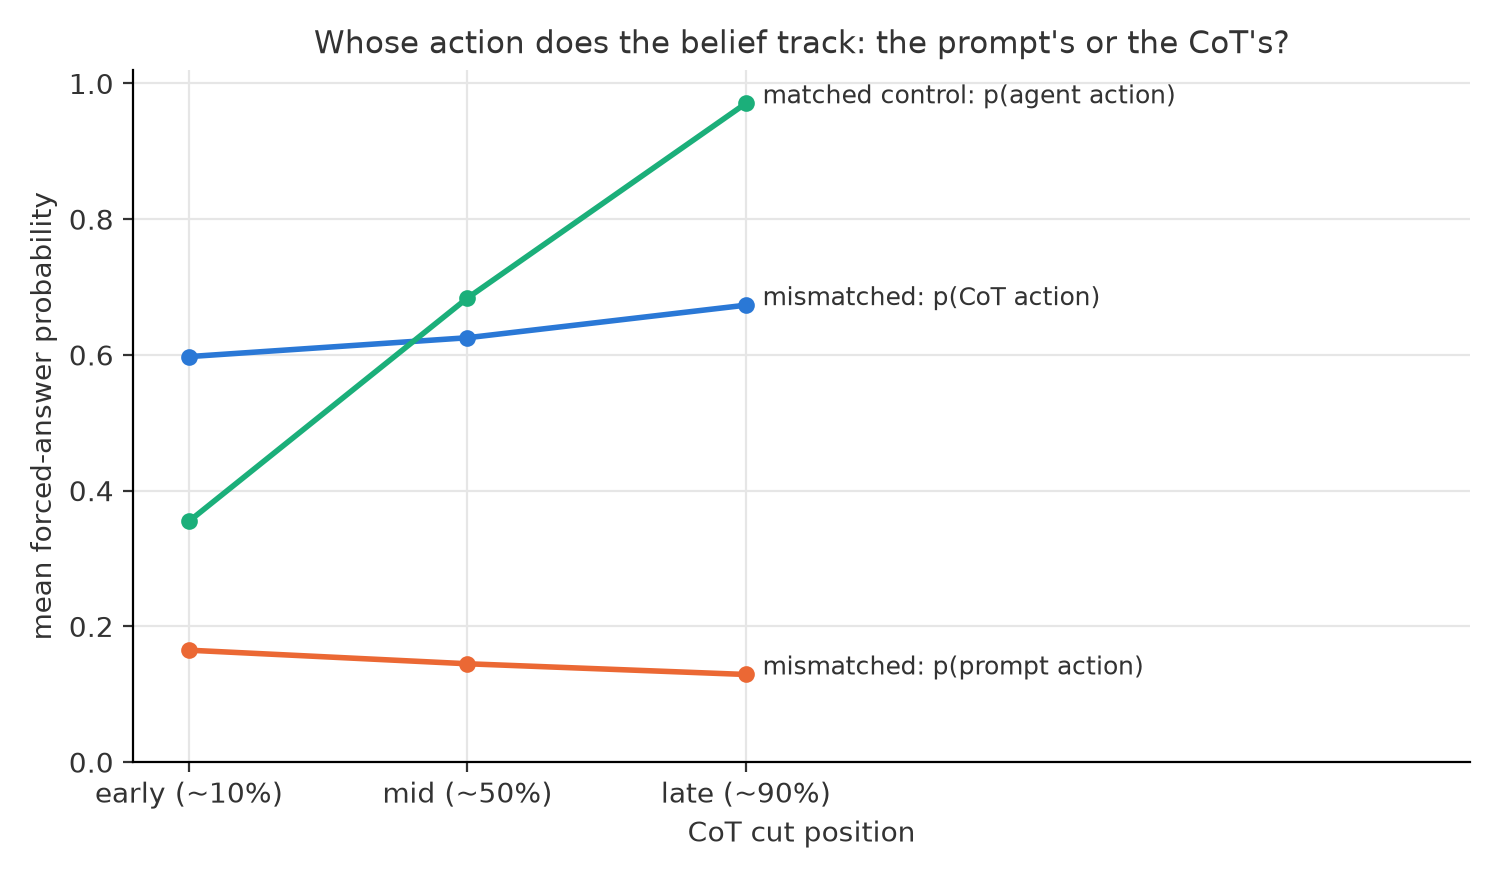
\includegraphics[width=\textwidth]{figures/counterfactual.png}
  \end{subfigure}
  \hfill
  \begin{subfigure}[b]{0.41\textwidth}
    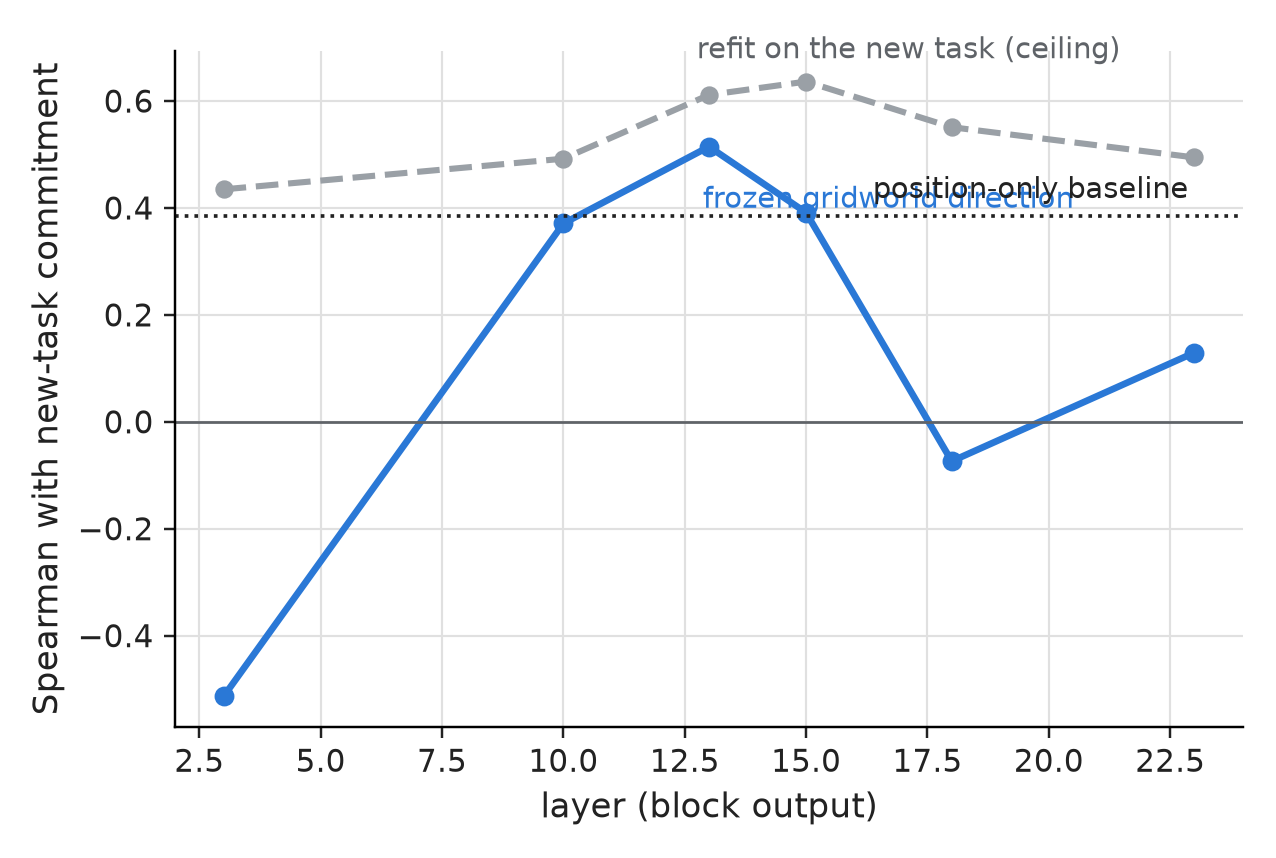
\includegraphics[width=\textwidth]{figures/transfer.png}
  \end{subfigure}
  \caption{\textbf{Left:} with the prompt of one decision and the reasoning of another, the
  belief follows the reasoning at every cut position. \textbf{Right:} a commitment
  direction frozen from gridworld data, applied without refitting to arithmetic chains of
  thought, against a positional bar and a refit-on-task ceiling.}
  \label{fig:counterfactual}
\end{figure}

\begin{figure}[t]
  \centering
  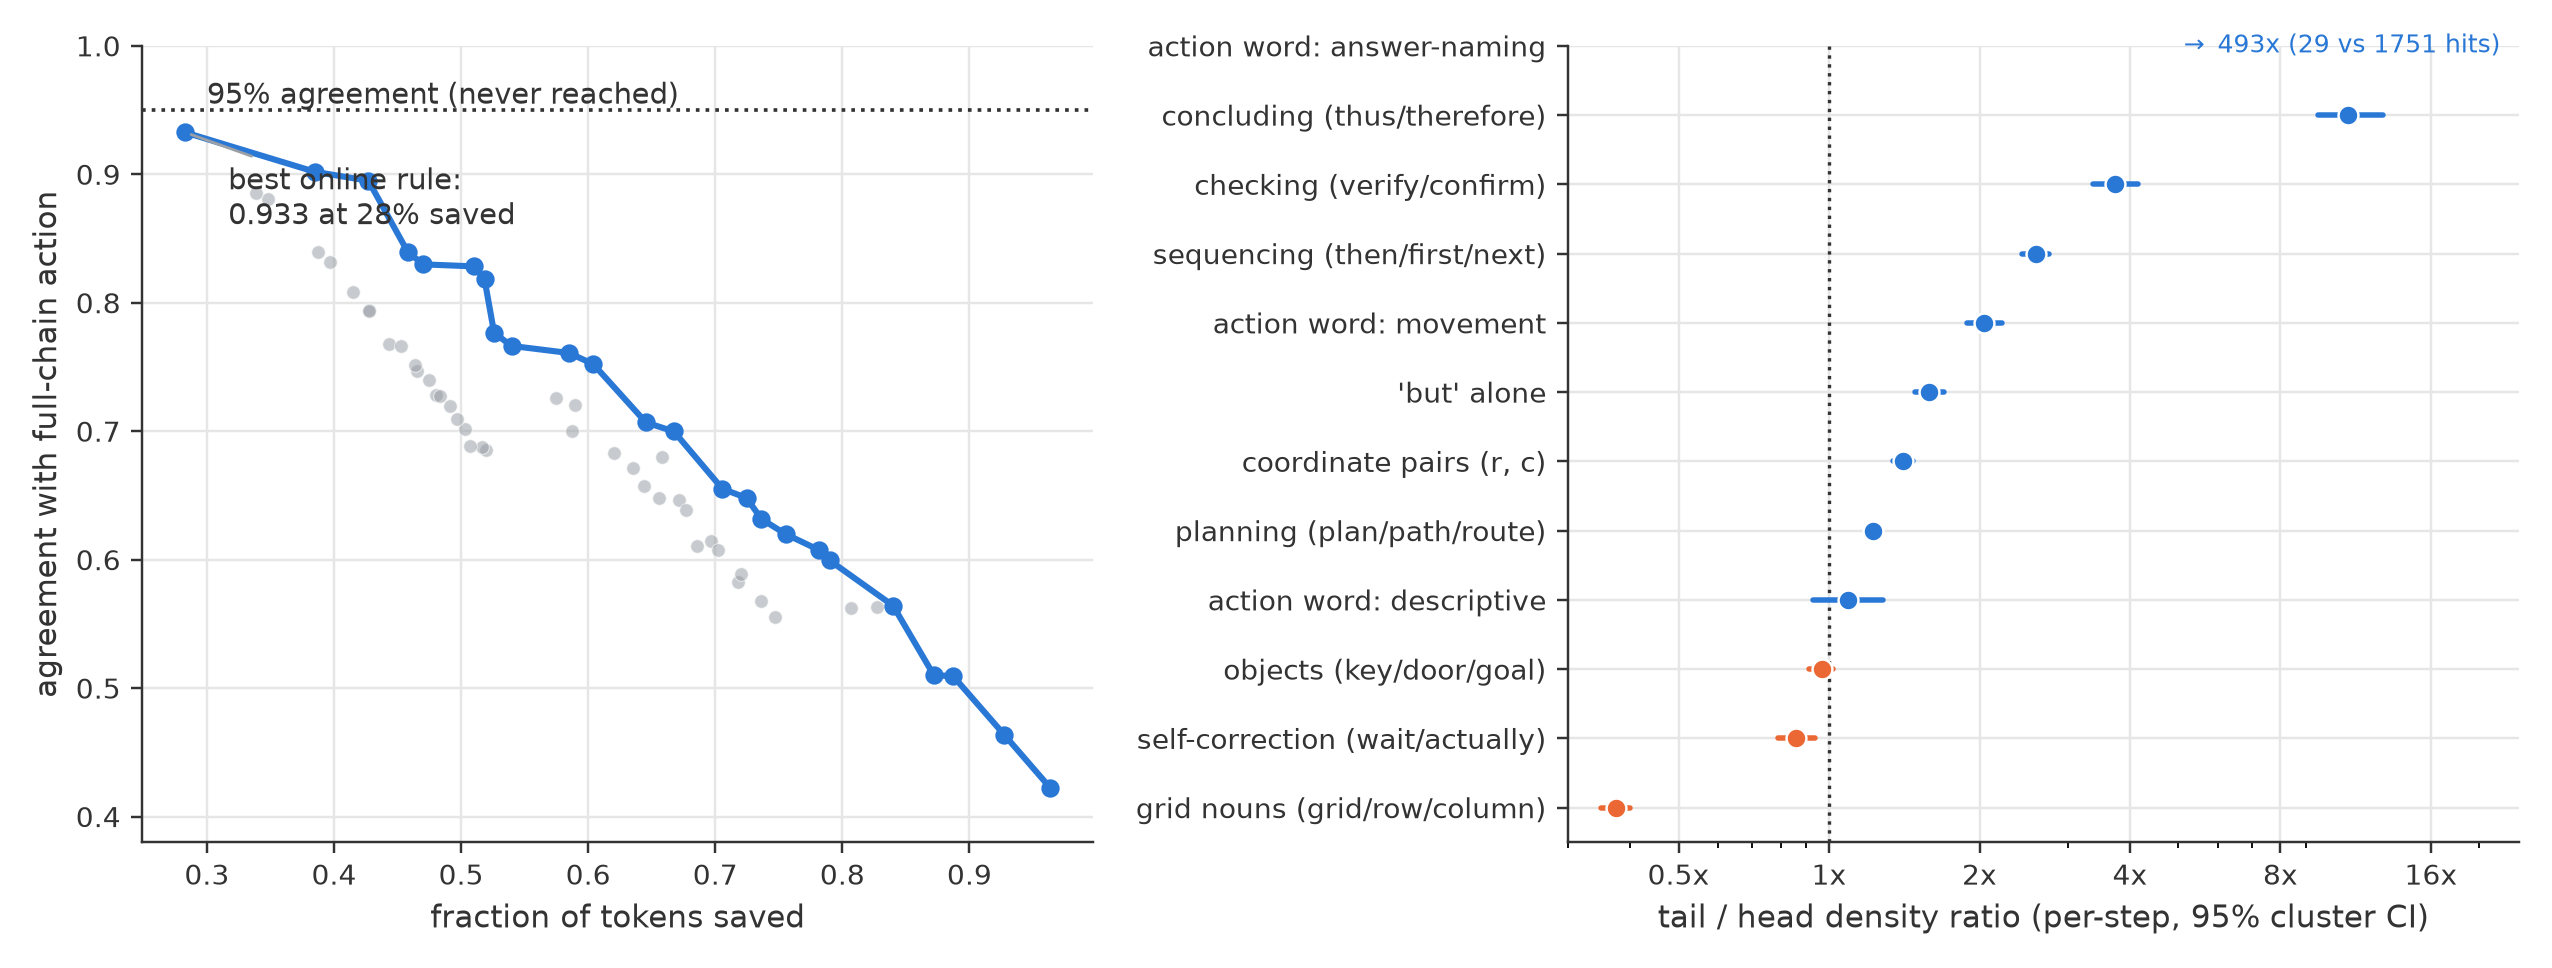
\includegraphics[width=0.98\textwidth]{figures/tail_v2.png}
  \caption{\textbf{Left:} accuracy versus token savings for 63 prospective early-exit rules,
  with the Pareto frontier highlighted; no online rule reaches $95\%$ agreement.
  \textbf{Right:} tail/head density ratios for the revised keyword classes (log scale;
  filled dots with $95\%$ trajectory-clustered CIs; blue rises, orange falls). Checking,
  sequencing, and coordinate language rise while grid nouns and self-correction fall;
  answer-naming uses of direction words are essentially absent before stabilisation.
  Event-aligned versions of these densities and all robustness checks are in
  Appendix~\ref{app:lexicon}.}
  \label{fig:tail}
\end{figure}

\bibliographystyle{plainnat}
\begin{thebibliography}{99}
\small

\bibitem[Bogdan et al.(2025)]{anchors2025}
P.~C. Bogdan et al.
\newblock Thought anchors: which LLM reasoning steps matter?
\newblock \emph{arXiv:2506.19143}, 2025.

\bibitem[Chen et al.(2026)]{boundary2026}
Anonymous.
\newblock Beyond the commitment boundary: probing epiphenomenal chain-of-thought in large
reasoning models.
\newblock \emph{arXiv:2606.13603}, 2026.

\bibitem[Kadavath et al.(2022)]{kadavath2022}
S.~Kadavath et al.
\newblock Language models (mostly) know what they know.
\newblock \emph{arXiv:2207.05221}, 2022.

\bibitem[Makelov et al.(2023)]{makelov2023}
A.~Makelov, G.~Lange, and N.~Nanda.
\newblock Is this the subspace you are looking for? An interpretability illusion for
subspace activation patching.
\newblock \emph{arXiv:2311.17030}, 2023.

\bibitem[McGrath et al.(2023)]{mcgrath2023}
T.~McGrath, M.~Rahtz, J.~Kramar, V.~Mikulik, and S.~Legg.
\newblock The Hydra effect: emergent self-repair in language model computations.
\newblock \emph{arXiv:2307.15771}, 2023.

\bibitem[Wang et al.(2023)]{wang2023ioi}
K.~Wang, A.~Variengien, A.~Conmy, B.~Shlegeris, and J.~Steinhardt.
\newblock Interpretability in the wild: a circuit for indirect object identification.
\newblock In \emph{ICLR}, 2023.

\bibitem[Rimsky et al.(2024)]{rimsky2024}
N.~Rimsky, N.~Gabrieli, J.~Schulz, M.~Tong, E.~Hubinger, and A.~M. Turner.
\newblock Steering Llama 2 via contrastive activation addition.
\newblock In \emph{ACL}, 2024.

\bibitem[Lanham et al.(2023)]{lanham2023}
T.~Lanham et al.
\newblock Measuring faithfulness in chain-of-thought reasoning.
\newblock \emph{arXiv:2307.13702}, 2023.

\bibitem[Meng et al.(2022)]{meng2022}
K.~Meng, D.~Bau, A.~Andonian, and Y.~Belinkov.
\newblock Locating and editing factual associations in GPT.
\newblock In \emph{NeurIPS}, 2022.

\bibitem[Shai et al.(2024)]{shai2024}
A.~S. Shai, S.~E. Marzen, L.~Teixeira, A.~G. Oldenziel, and P.~M. Riechers.
\newblock Transformers represent belief state geometry in their residual stream.
\newblock In \emph{NeurIPS}, 2024.

\bibitem[Turner et al.(2023)]{turner2023}
A.~M. Turner et al.
\newblock Activation addition: steering language models without optimization.
\newblock \emph{arXiv:2308.10248}, 2023.

\bibitem[Turpin et al.(2023)]{turpin2023}
M.~Turpin, J.~Michael, E.~Perez, and S.~R. Bowman.
\newblock Language models don't always say what they think.
\newblock In \emph{NeurIPS}, 2023.

\bibitem[Anonymous(2026a)]{commit2026}
Anonymous.
\newblock When does a language model commit? A finite-answer theory of pre-verbalization
commitment.
\newblock \emph{arXiv:2605.06723}, 2026.

\bibitem[Anonymous(2026b)]{broken2026}
Anonymous.
\newblock Why do LLMs struggle in strategic play? Broken links between observations,
beliefs, and actions.
\newblock \emph{arXiv:2605.00226}, 2026.

\bibitem[Anonymous(2026c)]{twostage2026}
Anonymous.
\newblock When models decide and when they bind: a two-stage computation for
multiple-choice question answering.
\newblock \emph{arXiv:2601.03914}, 2026.

\bibitem[Anonymous(2025)]{temporal2025}
Anonymous.
\newblock Temporal predictors of outcome in reasoning language models.
\newblock \emph{arXiv:2511.14773}, 2025.

\bibitem[Monroe et al.(2008)]{monroe2008}
B.~L. Monroe, M.~P. Colaresi, and K.~M. Quinn.
\newblock Fightin' words: Lexical feature selection and evaluation for
  identifying the content of political conflict.
\newblock \emph{Political Analysis}, 16(4):372--403, 2008.

\end{thebibliography}

\appendix

\section{Robustness of the tail lexical analysis}
\label{app:lexicon}

The published version of the Figure~\ref{fig:tail} lexical comparison used five ad-hoc
keyword classes with no validation. An audit found four flaws: the weighting convention
was unstated (per-decision ratios differ from character-pooled ones by up to a factor of
two); the ``verification'' class was $45\%$ the single conclusion marker ``thus''; the
``correction'' class was $77\%$ the word ``but'', and removing that one word
\emph{inverts} its direction; and the design could not distinguish
stabilisation-linked change from generic end-of-chain drift. This appendix documents the
corrected analysis that Section~4 now reports.

\paragraph{Design.} All statistics use the $1007$ of $1276$ decisions with more than
$200$ characters on each side of $\Tstab$. Ratios are reported under both weightings:
\emph{per-decision} (ratio of mean per-decision densities; the convention in the main
text) and \emph{character-pooled}; $95\%$ CIs come from resampling the $95$ trajectories
with replacement ($2000$ reps). Each multi-word class is re-estimated with every literal
left out in turn (LOO); a class is \emph{robust} iff its CI excludes $1$ and no LOO
variant flips its direction. Every class passed an author-labelled precision sample
($n = 16$--$20$ occurrences per class, labelled against a written codebook; regex classes
scored $1.00$, Wilson $95\%$ lower bounds $0.81$--$0.84$). The event-aligned analysis
measures each class's density in $400$-character windows around the stabilisation
character position; the placebo redraws each chain's stabilisation point from another
chain in the same length quintile ($200$ draws), which preserves the marginal position
distribution while destroying the alignment to the decision.

\begin{table}[h]
  \centering
  \caption{Revised keyword classes. Jump $p$ is the two-sided empirical probability of
  the observed density jump at $\Tstab$ under the shuffled-stabilisation placebo;
  ``at $\Tstab$'' marks stabilisation-linked change, ``end'' marks a class with no
  excess jump at $\Tstab$ (its rise is anchored to the chain end; for conclusion
  markers the jump at $\Tstab$ is in fact significantly \emph{below} placebo).}
  \label{tab:lexicon}
  \small
  \begin{tabular}{lccccc}
    \toprule
    class & per-decision & pooled & LOO range & jump $p$ & timing \\
    \midrule
    checking & $3.73$ $[3.37, 4.15]$ & $2.16$ & $[3.46, 16.0]$ & $0.01$ & at $\Tstab$ \\
    concluding (thus/therefore) & $10.9$ $[9.50, 12.8]$ & $3.69$ & $[5.65, 11.4]$ & $0.01$ & end \\
    sequencing (then/first/next) & $2.60$ $[2.44, 2.75]$ & $1.96$ & $[2.33, 3.06]$ & $0.01$ & at $\Tstab$ \\
    coordinate pairs & $1.41$ $[1.34, 1.47]$ & $1.21$ & --- & $0.01$ & at $\Tstab$ \\
    planning (plan/path/route) & $1.23$ $[1.18, 1.27]$ & $1.20$ & $[1.09, 1.51]$ & $0.07$ & --- \\
    objects (key/door/goal) & $0.97$ $[0.91, 1.02]$ & $1.06$ & $[0.88, 1.03]$ & $0.01$ & at $\Tstab$ ($+$) \\
    self-correction (no ``but'') & $0.86$ $[0.79, 0.94]$ & $0.94$ & $[0.83, 0.99]$ & $0.38$ & --- \\
    grid nouns & $0.37$ $[0.35, 0.40]$ & $0.55$ & $[0.24, 0.50]$ & $0.01$ & at $\Tstab$ \\
    \bottomrule
  \end{tabular}
\end{table}

\begin{figure}[h]
  \centering
  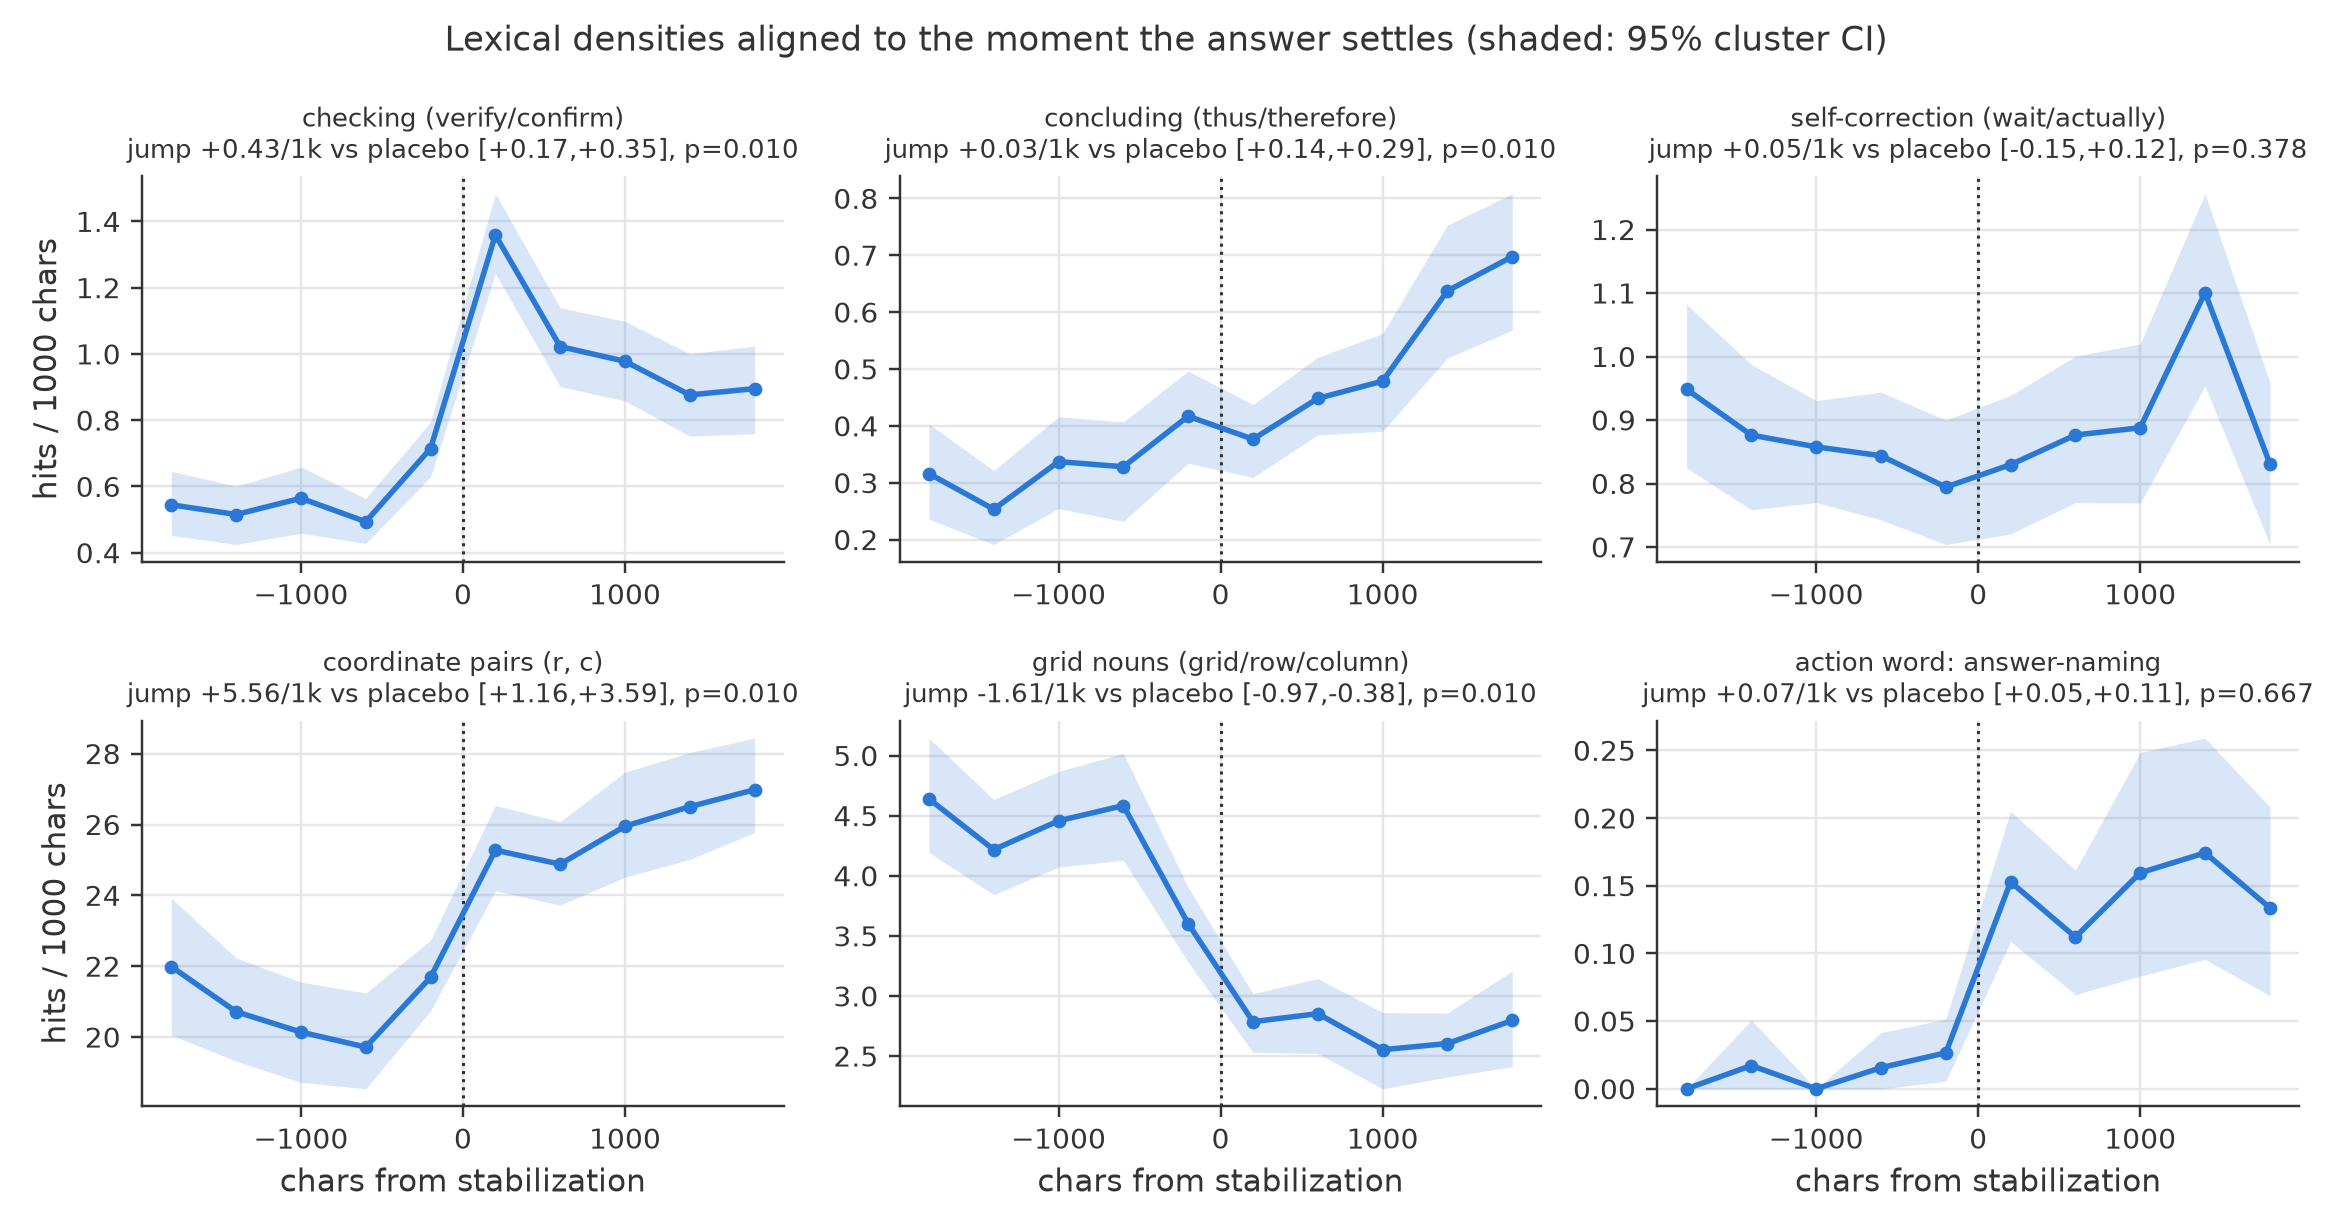
\includegraphics[width=0.98\textwidth]{figures/tail_event_aligned.png}
  \caption{Densities aligned to the stabilisation moment (shaded: $95\%$
  trajectory-clustered CIs). Checking spikes and grid nouns collapse \emph{at} the
  decision; conclusion markers drift up smoothly toward the end of the chain with no
  excess at $\Tstab$; self-correction is flat. The decision is visible in the text as a
  switch from parsing the world to walking the solution.}
  \label{fig:eventaligned}
\end{figure}

\begin{figure}[h]
  \centering
  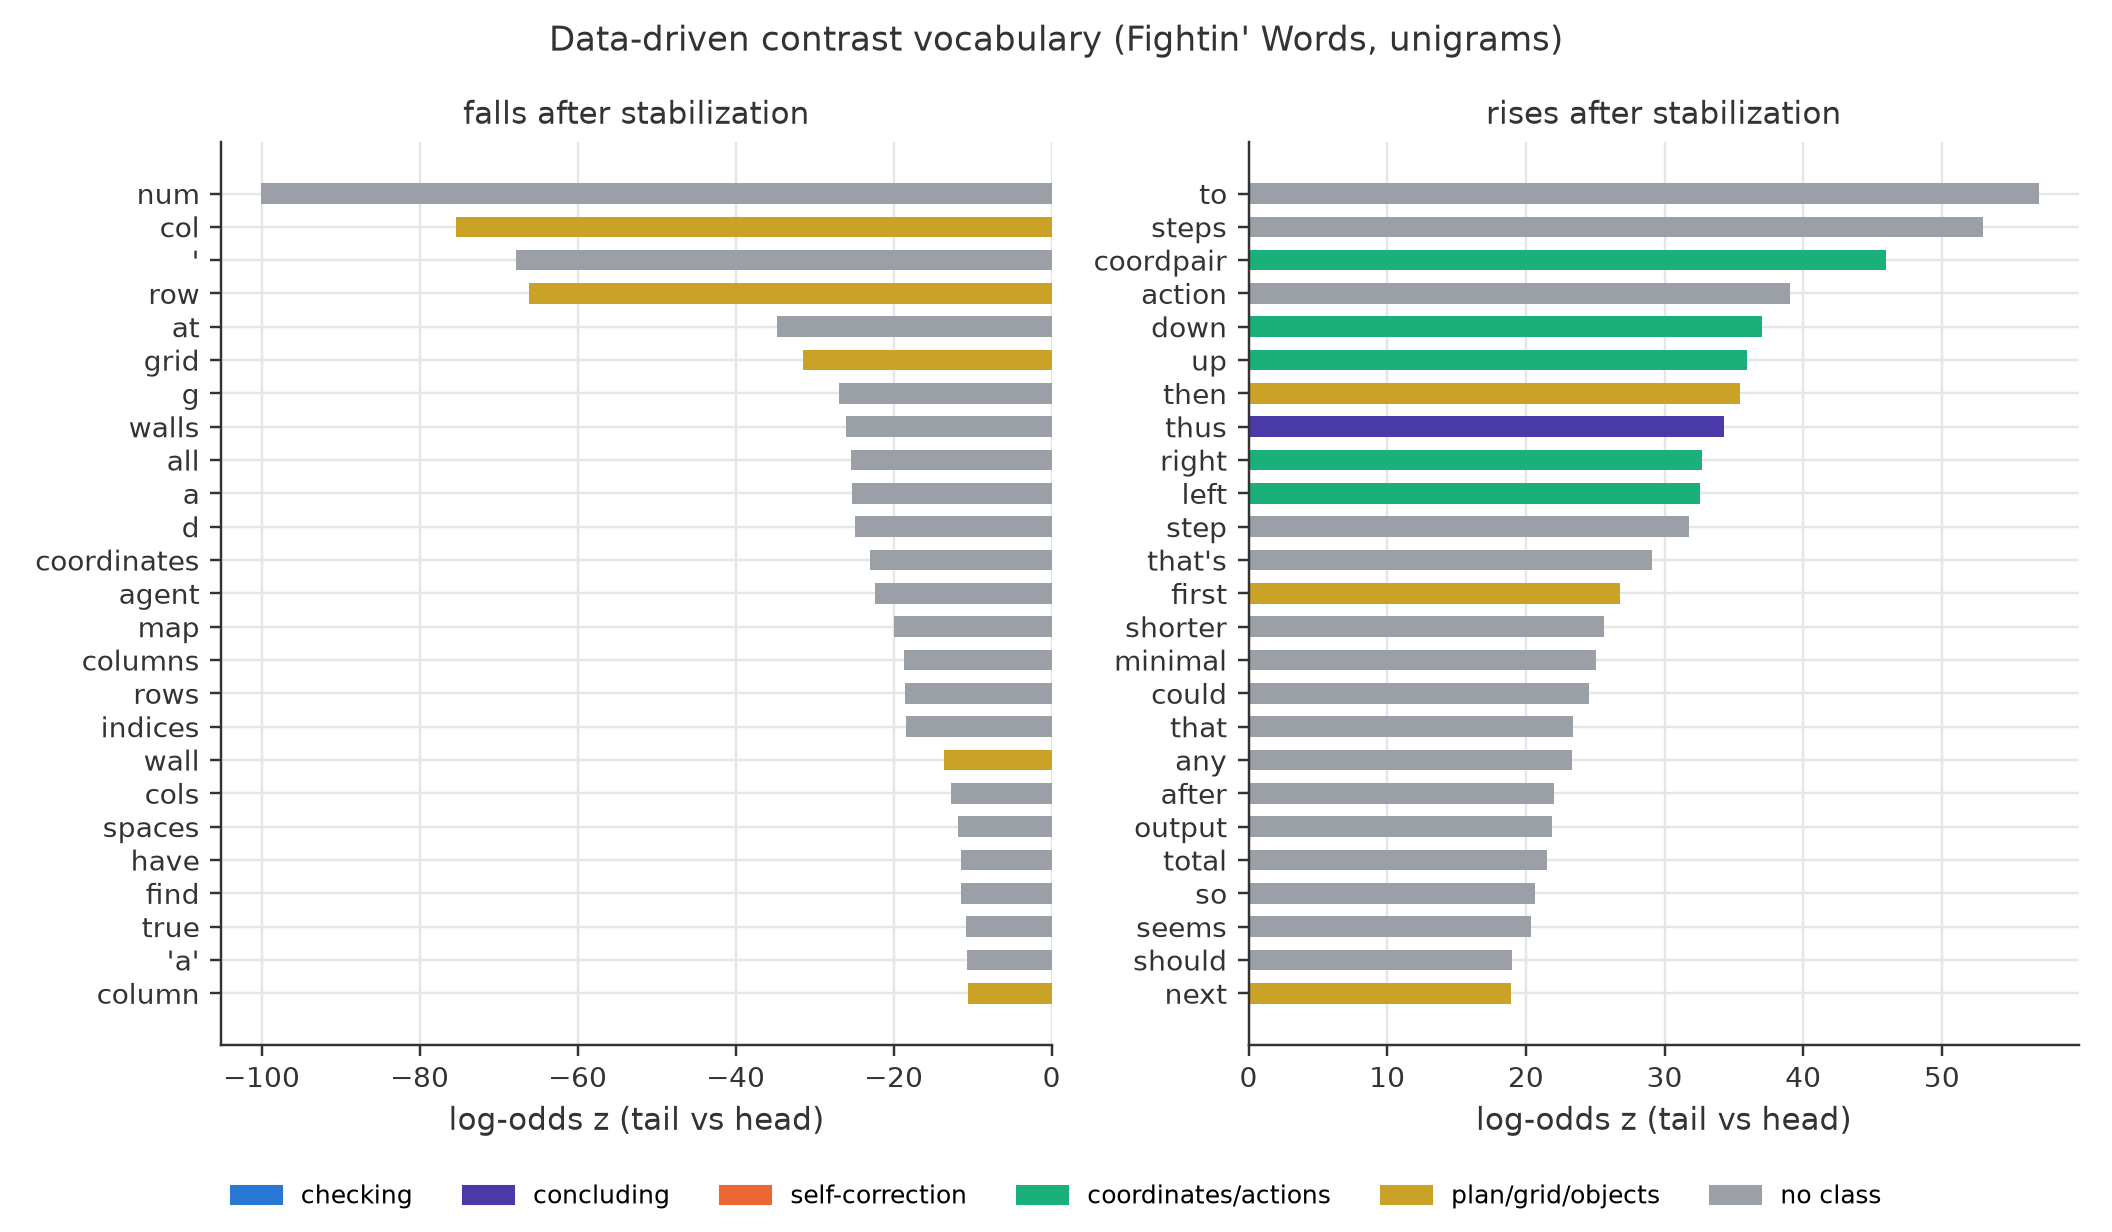
\includegraphics[width=0.9\textwidth]{figures/tail_fightin_words.png}
  \caption{Data-driven contrast vocabulary \citep{monroe2008}: the $25$ unigrams that
  rise and fall most after stabilisation ($z$-scores of informative-Dirichlet log-odds;
  ``coordpair'' and ``num'' are normalised coordinate pairs and numerals). No keyword
  list is assumed; the discovered terms are then coloured by which revised class, if
  any, contains them. Of the top-$25$ rising terms, all stay in the top $50$ in at
  least $93\%$ of trajectory bootstrap resamples except ``should'' ($76\%$) and
  ``next'' ($60\%$).}
  \label{fig:fightin}
\end{figure}

\paragraph{Embedding soft categories mostly failed validation.} As a paraphrase-robust
complement we also scored every sentence by cosine similarity to seed-phrase centroids
(all-MiniLM-L6-v2) for six semantic classes. The author-labelled precision sample
rejected four of the six: top-decile ``checking'' sentences were mostly short imperatives
containing coordinates (precision $0.13$), ``self-correction'' was dominated by
topically-similar but non-corrective sentences (precision $0.06$; sentence encoders are
poor at negation), and ``answer-naming'' scored $0.25$. Only ``planning'' ($0.88$) and
``spatial-description'' ($0.88$) passed, and both agree with the keyword result
(planning-talk rises modestly; world-description falls, jump beyond placebo at
$\Tstab$). We therefore cite only these two, and report the failure itself: unvalidated
embedding-similarity categories can manufacture findings --- the raw
``self-correction'' soft score \emph{rises} after stabilisation ($p < 10^{-4}$) while
actual correction markers fall.

\paragraph{A sentence-function annotator fared little better.} We also labelled all
$16{,}640$ sentences of a $120$-decision subsample with an eight-way reasoning-function
taxonomy adapted from \citet{anchors2025}, using the subject model itself
(greedy, fixed prompt, local) as annotator, and validated against $152$ blind
author-labelled sentences. The pre-declared gate (Cohen's $\kappa \ge 0.6$) \emph{failed}
($\kappa = 0.50$): only \emph{answering} ($1.00$ precision), \emph{concluding} ($0.95$)
and \emph{parsing} ($0.84$) are usable, while \emph{verifying} ($0.21$) and
\emph{planning} ($0.42$) collapse into boundary confusions. The three reliable classes
independently corroborate Section~4: parsing sentences fall from $56\%$ to $14\%$ of
the chain (event-aligned drop at $\Tstab$, $p = 0.02$ versus placebo), answer-naming is
tail-exclusive, and concluding is end-anchored (no excess at $\Tstab$, $p = 0.38$).
The verification claim rests on the validated keyword class, not on either automatic
annotator.

\end{document}
